\documentclass[11pt,a4paper]{article}

\usepackage[margin=1in]{geometry}
\usepackage{amsmath,amssymb,bm}
\usepackage{natbib}
\usepackage{hyperref}
\usepackage{booktabs}
\usepackage{enumitem}
\usepackage{titlesec}
\usepackage{graphicx}
\usepackage{fancyhdr}
\usepackage{tikz}
\usetikzlibrary{arrows.meta,positioning,fit,backgrounds,calc,shapes.geometric}

% --- Architecture-schematic palette + node styles (Fig. legoESM stack) ---
\definecolor{legocore}{RGB}{55,71,79}      % substrate (slate)
\definecolor{legoatm}{RGB}{30,136,229}     % atmosphere (blue)
\definecolor{legoocn}{RGB}{0,137,123}      % ocean (teal)
\definecolor{legolnd}{RGB}{124,179,66}     % land (green)
\definecolor{legoice}{RGB}{0,172,193}      % ice (cyan)
\definecolor{legoorc}{RGB}{142,36,170}     % orchestration (purple)
\definecolor{legoml}{RGB}{244,143,177}     % ml accent (pink)
\definecolor{legoflow}{RGB}{239,108,0}     % data-flow accent (orange)
\tikzset{
  lbox/.style={rounded corners=2pt,draw,thick,align=center,font=\footnotesize,
               inner sep=4pt,minimum height=8mm,text=white},
  llabel/.style={font=\scriptsize\itshape,text=black!70},
  lego/.style={draw,thick,rounded corners=2pt,align=center,font=\scriptsize,
               inner sep=3pt,minimum height=7mm,fill=white},
  dep/.style={-{Stealth[length=2mm]},draw=black!55,thick},
  flow/.style={-{Stealth[length=2.5mm]},draw=legoflow,very thick},
}

\pagestyle{fancy}
\fancyhead[L]{\small legoESM Technical Documentation}
\fancyhead[R]{\small\thepage}
\fancyfoot{}

\titleformat{\section}{\Large\bfseries}{}{0em}{}
\titleformat{\subsection}{\large\bfseries}{}{0em}{}
\titleformat{\subsubsection}{\normalsize\bfseries}{}{0em}{}

\newcommand{\dd}{\mathrm{d}}
\newcommand{\pp}{\partial}
\newcommand{\half}{\tfrac{1}{2}}
\newcommand{\Rd}{R_d}
\newcommand{\cpd}{c_p}
\newcommand{\Lv}{L_v}
\newcommand{\Rv}{R_v}
\newcommand{\pref}{p_0}
\newcommand{\SB}{\sigma_{\mathrm{SB}}}
\DeclareMathOperator{\Var}{Var}

% Document version tracks the package MAJOR.MINOR (root pyproject [project].version).
\newcommand{\legoesmversion}{1.0}
\title{\textbf{legoESM \legoesmversion{}: A Differentiable Earth System Model in JAX}\\[6pt]
\large Technical Documentation of Equations and Implementations}
\author{legoESM Development Team}
\date{Version \legoesmversion{} --- October 2026}

\begin{document}

\maketitle
\tableofcontents
\newpage

%=============================================================================
\section{Introduction}
%=============================================================================

legoESM is a modular Earth System Model written entirely in JAX, supporting automatic differentiation through all components.  The model couples atmospheric, oceanic, land, sea-ice, and biogeochemical components on the sphere, with 25+ dynamical cores spanning five discretisation families (C-D grid FV3, finite-volume PPM, pseudospectral, FC-Gram, C-grid) and 35+ physics parameterisations.  The cubed-sphere implementation is unified around a single FV3-style C-D grid discretisation (Lin 2004, Putman \& Lin 2007) shared by atmosphere (shallow water, hydrostatic PE, non-hydrostatic CE) and ocean, eliminating the Hollingsworth--Kallberg instability.  The cubed-sphere transport uses an FV3-faithful PPM reconstruction with monotonicity limiters and flux-form mass transport on staggered grids, complemented by an FV3-style forward--backward shallow-water core (\texttt{fv3\_sw\_core.py}) implementing the full c\_sw/d\_sw stepping (kernels certified bit-exact against Fortran; full-chain fidelity in progress) and d2a2c\_vect (D-grid $\to$ A-grid $\to$ C-grid) vector conversion with duo-grid sub-grid metrics ($\sin\alpha_{\mathrm{sg}}$, $\cos\alpha_{\mathrm{sg}}$) following Mouallem et al.\ (2023).  The model includes a land carbon cycle with Farquhar photosynthesis and stomatal conductance, ocean biogeochemistry (abiotic carbon + NPZD ecosystem), sea-ice dynamics with EVP rheology and multi-category ice, CMIP6-class infrastructure (table-driven CF/CMOR output across eleven CMIP6 tables, experiment templates, restart reproducibility, documented tuning), and a fully differentiable 4D-Var data assimilation system leveraging JAX autodiff for adjoint-free gradient computation.  The MPI-distributed runtime supports native 4D halo exchange (one message per neighbour for all vertical levels), reverse-mode AD through MPI via a custom \texttt{sendrecv} VJP wrapper, and AD-safe \texttt{allreduce(SUM)} for gradient-compatible global reductions.  The codebase comprises approximately 990 source modules (${\sim}$590,000 lines of code, excluding the vendored CLM-ML canopy backend) exercised by roughly 32,000 test functions across some 2,700 test files.

\paragraph{What legoESM 1.0 adds.}
Version 1.0 is the first release in which a production climate configuration, rather than only the component library, is a versioned part of the model.  The headline additions since the previous documentation release are:
\begin{itemize}[nosep]
  \item a \textbf{production AMIP configuration} on the MPAS Voronoi mesh with a CAM6-homogenised physics suite --- CAM6 32-level hybrid table, Zhang--McFarlane convection, prognostic CLUBB with CAM6 cloud fraction, MG2-flavour two-moment microphysics, McICA cloud overlap, and an interactive multilayer land (Section~\ref{sec:amip-production});
  \item \textbf{conservation repairs}: on the production lane, conservative tracer vertical transport on the hybrid coordinate and column-conserving tracer positivity on every grid; in the spectral core, Simmons--Burridge vertical transport and frictional heating; and a single temperature-dependent latent-heat family used by the surface-flux interface, sea ice and the land canopy (schemes ported from a reference model, and the FV3 duo-grid lane, keep their own constants) (Sections~\ref{sec:conservation-v1} and~\ref{sec:constants});
  \item a hardened \textbf{parallel runtime} for multi-GPU and multi-node runs, with size-aware halo scheduling, space-filling-curve ordering, a communication-free ocean preconditioner, and explicit precision policies (Section~\ref{sec:parallel});
  \item an \textbf{FV3 duo-grid lane} whose adiabatic deck is certified against the Fortran FV3 core (Section~\ref{sec:fv3duo});
  \item table-driven \textbf{CMIP6 output} read from the official CMOR tables, with interval means and multi-rank output on the MPAS lane (Section~\ref{sec:cmip});
  \item unified \textbf{training and calibration lanes} that train one model registry across the WeatherBench and AIMIP campaigns and refuse parameters that carry no gradient (Section~\ref{sec:training}).
\end{itemize}

\paragraph{Design principles.}
\begin{itemize}[nosep]
  \item Pure-JAX implementation: all components are compatible with \texttt{jit}, \texttt{grad}, and \texttt{vmap}.
  \item Modular physics: each parameterisation follows a factory pattern returning a callable \texttt{physics\_fn(state, grid, coord) $\to$ Tendencies}.
  \item Multiple dynamical cores share the same physics interface, enabling interchangeable experiments.
  \item Neural-network components (SFNO) integrate seamlessly via the same JAX computational graph.
\end{itemize}

%=============================================================================
\section{Model Architecture}
%=============================================================================

legoESM is organised as a \emph{federation} of eight independently installable
packages that all ship into one shared \texttt{legoesm} PEP-420 namespace, layered
as an acyclic dependency graph whose import boundaries are enforced by
zero-ignore \texttt{lint-imports} contracts (Fig.~\ref{fig:dag}).  A single
\texttt{legoesm-core} substrate provides fields, grids, vertical coordinates,
operators, the device/precision runtime, the parallel halo/reduction layer, and
the grid\,$\times$\,complexity capability matrix; the four Earth-system components
(\texttt{atmosphere}, \texttt{ocean}, \texttt{land}, \texttt{ice}) depend
\emph{only} on the substrate and never on each other, so each can be
\texttt{pip install}ed and gradient-checked in isolation.  Above them sits an
orchestration cluster --- \texttt{coupler}+\texttt{driver},
\texttt{ml}+\texttt{training}+\texttt{da}, and \texttt{tools} --- whose mutual
edges form a uv-workspace cycle, so the three install together.

\begin{figure}[t]
\centering
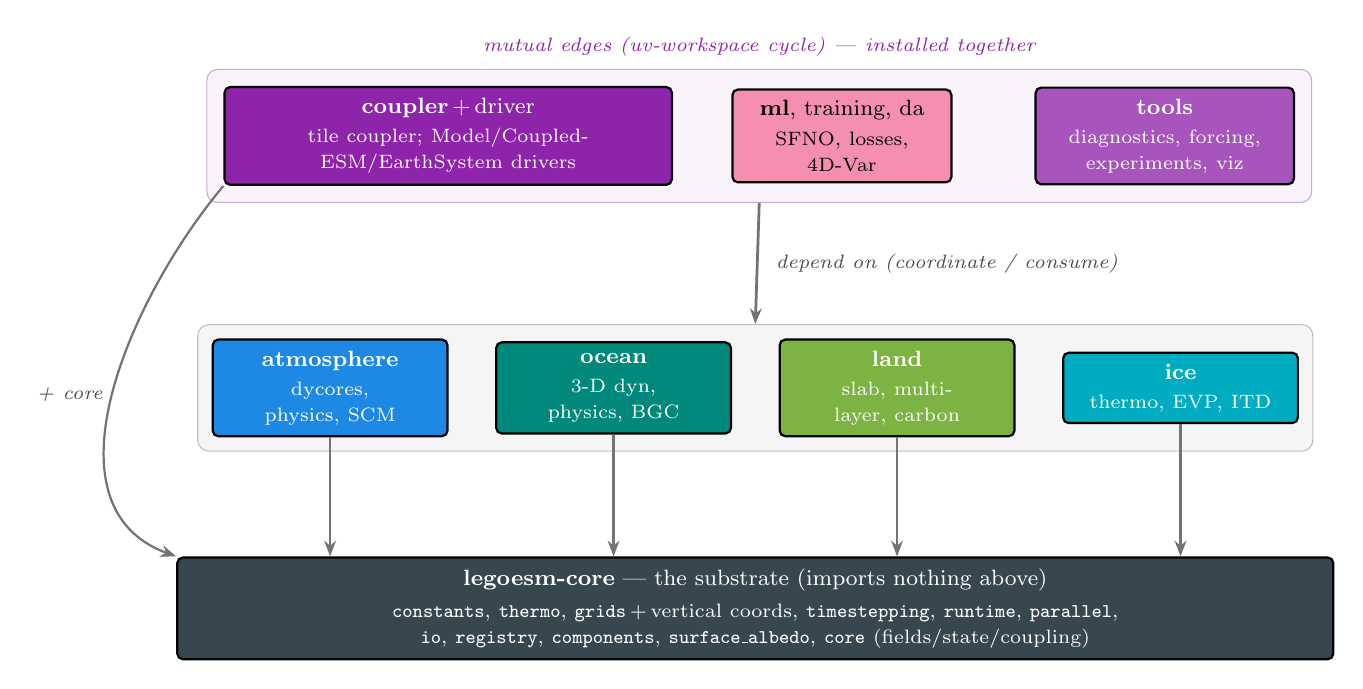
\begin{tikzpicture}
% substrate
\node[lbox,fill=legocore,text width=14.4cm,minimum height=12mm] (core) at (0,0)
 {\textbf{legoesm-core} --- the substrate (imports nothing above)\\[2pt]
  \scriptsize \texttt{constants}, \texttt{thermo}, \texttt{grids}\,+\,vertical coords, \texttt{timestepping}, \texttt{runtime}, \texttt{parallel}, \texttt{io}, \texttt{registry}, \texttt{components}, \texttt{surface\_albedo}, \texttt{core} (fields/state/coupling)};
% components
\node[lbox,fill=legoatm,text width=2.7cm] (atm) at (-5.4,2.8) {\textbf{atmosphere}\\[1pt]\scriptsize dycores, physics, SCM};
\node[lbox,fill=legoocn,text width=2.7cm] (ocn) at (-1.8,2.8) {\textbf{ocean}\\[1pt]\scriptsize 3-D dyn, physics, BGC};
\node[lbox,fill=legolnd,text width=2.7cm] (lnd) at (1.8,2.8) {\textbf{land}\\[1pt]\scriptsize slab, multilayer, carbon};
\node[lbox,fill=legoice,text width=2.7cm] (ice) at (5.4,2.8) {\textbf{ice}\\[1pt]\scriptsize thermo, EVP, ITD};
% orchestration cluster
\node[lbox,fill=legoorc,text width=5.4cm] (coup) at (-3.9,6.0) {\textbf{coupler}\,+\,driver\\[1pt]\scriptsize tile coupler; Model/Coupled\-ESM/EarthSystem drivers};
\node[lbox,fill=legoml,text=black,text width=2.5cm] (ml) at (1.1,6.0) {\textbf{ml}, training, da\\[1pt]\scriptsize SFNO, losses, 4D-Var};
\node[lbox,fill=legoorc!78,text width=3.0cm] (tools) at (5.2,6.0) {\textbf{tools}\\[1pt]\scriptsize diagnostics, forcing, experiments, viz};
% component -> core (depends on)
\draw[dep] (atm.south) -- (atm.south|-core.north);
\draw[dep] (ocn.south) -- (ocn.south|-core.north);
\draw[dep] (lnd.south) -- (lnd.south|-core.north);
\draw[dep] (ice.south) -- (ice.south|-core.north);
\begin{scope}[on background layer]
\node[draw=black!25,rounded corners,fill=black!4,fit=(atm)(ice),inner sep=5pt] (compband){};
\node[draw=legoorc!40,rounded corners,fill=legoorc!5,fit=(coup)(ml)(tools),inner sep=6pt] (orcband){};
\end{scope}
\draw[dep,line width=1pt] (orcband.south) -- node[llabel,right,xshift=1mm]{depend on (coordinate / consume)} (compband.north);
\draw[dep] (coup.south west) to[out=-130,in=160] node[llabel,left]{+ core} (core.north west);
\node[llabel,above=1pt of orcband.north,text=legoorc] {\scriptsize mutual edges (uv-workspace cycle) --- installed together};
\end{tikzpicture}
\caption{\textbf{Federation dependency DAG.} Arrows point from a package to what
it imports (``depends on''); the layering is gated by zero-ignore import
contracts (see \texttt{FEDERATION.md}). The four components are mutually
independent and standalone-installable (contract \#2); the orchestration cluster
(coupler\,/\,ml\,/\,tools) sits above and carries the only mutual edges.}
\label{fig:dag}
\end{figure}

The ``lego'' in legoESM is the second design axis: standard tensor-in /
tendency-out interfaces let every block --- dynamical core, each physics
parameterisation, grid, vertical coordinate, time integrator, and even
classical-versus-neural physics --- be swapped independently by a string scheme
name resolved through a factory (Table~\ref{tab:dials}).
Figure~\ref{fig:flow} traces one coupled time step through these swap points.

\begin{figure}[p]
\centering
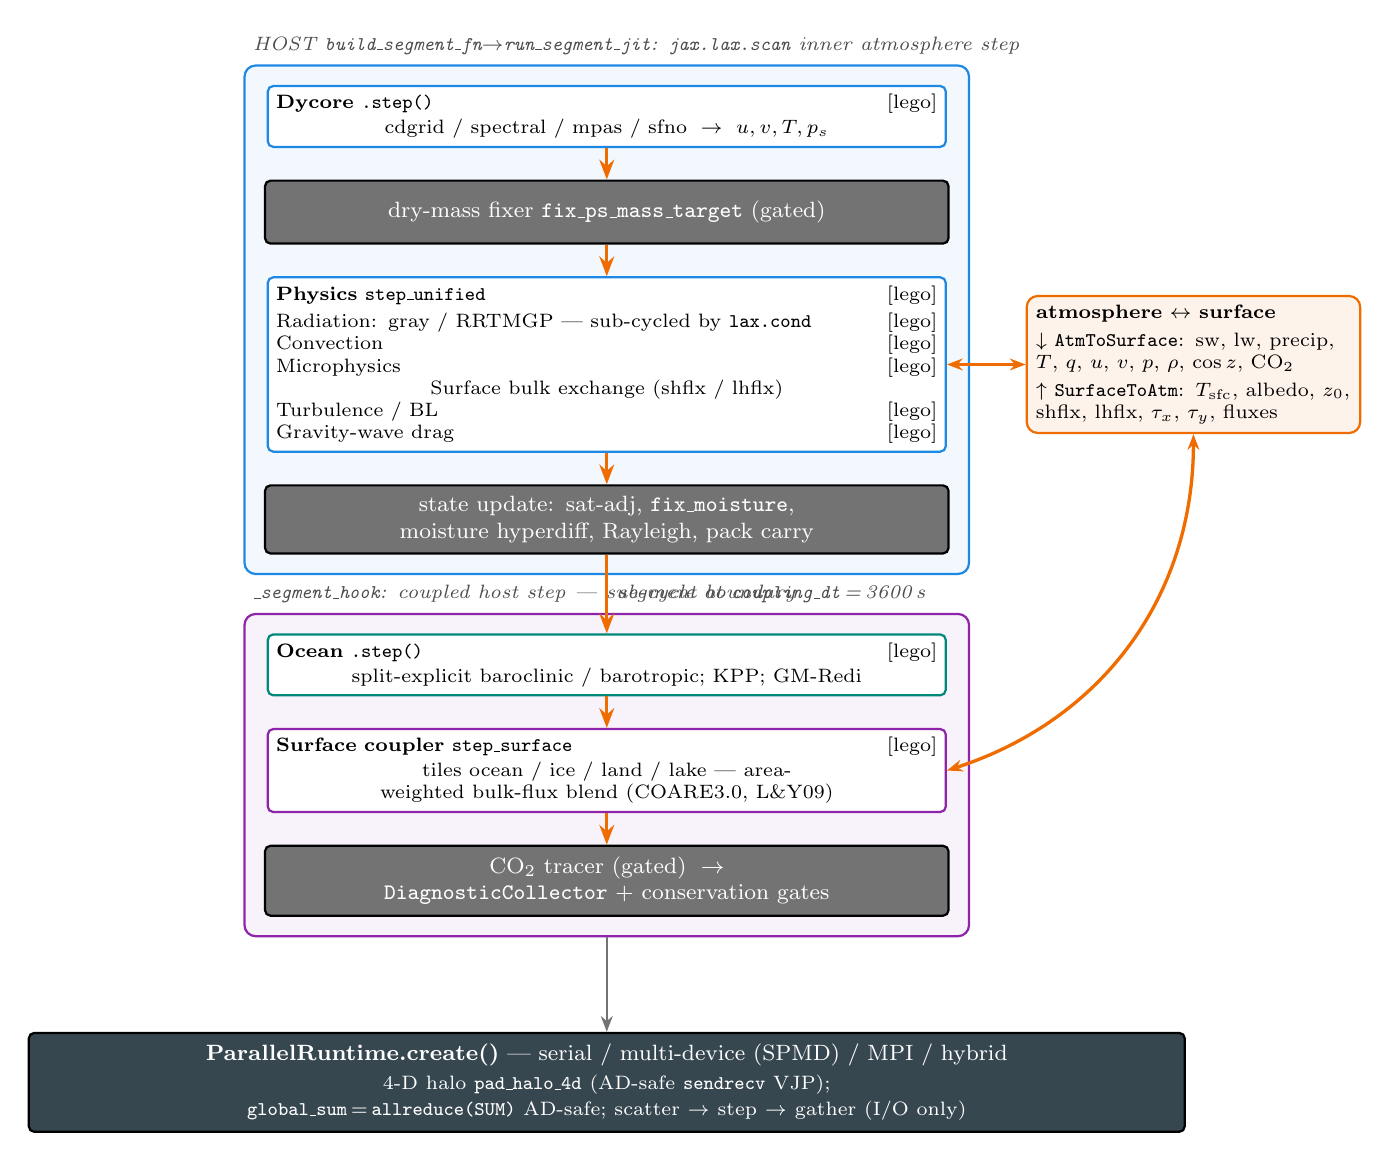
\begin{tikzpicture}[node distance=4mm]
% --- atmosphere inner step ---
\node[lego,draw=legoatm,text width=8.4cm] (dyc) at (0,0)
 {\textbf{Dycore} \texttt{.step()}\hfill[lego]\\[1pt]
  cdgrid / spectral / mpas / sfno \;$\to$\; $u,v,T,p_s$};
\node[lbox,fill=black!55,text width=8.4cm,below=of dyc] (mfix)
 {dry-mass fixer \texttt{fix\_ps\_mass\_target} (gated)};
\node[lego,draw=legoatm,text width=8.4cm,below=of mfix] (phys)
 {\textbf{Physics} \texttt{step\_unified}\hfill[lego]\\[2pt]
  Radiation: gray / RRTMGP --- sub-cycled by \texttt{lax.cond}\hfill[lego]\\
  Convection\hfill[lego]\\
  Microphysics\hfill[lego]\\
  Surface bulk exchange (shflx / lhflx)\\
  Turbulence / BL\hfill[lego]\\
  Gravity-wave drag\hfill[lego]};
\node[lbox,fill=black!55,text width=8.4cm,below=of phys] (supd)
 {state update: sat-adj, \texttt{fix\_moisture}, moisture hyperdiff, Rayleigh, pack carry};
% --- coupled host step ---
\node[lego,draw=legoocn,text width=8.4cm,below=10mm of supd] (ocn)
 {\textbf{Ocean} \texttt{.step()}\hfill[lego]\\[1pt]
  split-explicit baroclinic / barotropic; KPP; GM-Redi};
\node[lego,draw=legoorc,text width=8.4cm,below=of ocn] (surf)
 {\textbf{Surface coupler} \texttt{step\_surface}\hfill[lego]\\[1pt]
  tiles ocean / ice / land / lake --- area-weighted bulk-flux blend (COARE3.0, L\&Y09)};
\node[lbox,fill=black!55,text width=8.4cm,below=of surf] (co2)
 {CO$_2$ tracer (gated) \;$\to$\; \texttt{DiagnosticCollector} + conservation gates};
% loop containers
\begin{scope}[on background layer]
\node[draw=legoatm,thick,rounded corners,fill=legoatm!6,fit=(dyc)(supd),inner sep=7pt] (atmloop){};
\node[draw=legoorc,thick,rounded corners,fill=legoorc!6,fit=(ocn)(co2),inner sep=7pt] (cploop){};
\end{scope}
\node[llabel,anchor=south west] at (atmloop.north west) {HOST \texttt{build\_segment\_fn}$\to$\texttt{run\_segment\_jit}: \texttt{jax.lax.scan} inner atmosphere step};
\node[llabel,anchor=south west] at (cploop.north west) {\texttt{\_segment\_hook}: coupled host step --- sub-cycle at \texttt{coupling\_dt}\,=\,3600\,s};
% flow arrows
\draw[flow] (dyc) -- (mfix);
\draw[flow] (mfix) -- (phys);
\draw[flow] (phys) -- (supd);
\draw[flow] (supd) -- (ocn) node[midway,llabel,right]{segment boundary};
\draw[flow] (ocn) -- (surf);
\draw[flow] (surf) -- (co2);
% atm<->surface exchange
\node[draw=legoflow,thick,rounded corners,fill=legoflow!8,text width=4.0cm,right=10mm of phys,align=left,font=\scriptsize] (exch)
 {\textbf{atmosphere $\leftrightarrow$ surface}\\[2pt]
  $\downarrow$ \texttt{AtmToSurface}: sw, lw, precip, $T$, $q$, $u$, $v$, $p$, $\rho$, $\cos z$, CO$_2$\\[2pt]
  $\uparrow$ \texttt{SurfaceToAtm}: $T_{\mathrm{sfc}}$, albedo, $z_0$, shflx, lhflx, $\tau_x$, $\tau_y$, fluxes};
\draw[{Stealth[length=2mm]}-{Stealth[length=2mm]},draw=legoflow,very thick] (phys.east) -- (exch.west);
\draw[{Stealth[length=2mm]}-{Stealth[length=2mm]},draw=legoflow,very thick] (surf.east) to[out=18,in=-90] (exch.south);
% parallel substrate
\node[lbox,fill=legocore,text width=14.4cm,below=12mm of cploop.south,anchor=north] (par)
 {\textbf{ParallelRuntime.create()} --- serial / multi-device (SPMD) / MPI / hybrid\\[1pt]
  \scriptsize 4-D halo \texttt{pad\_halo\_4d} (AD-safe \texttt{sendrecv} VJP); \texttt{global\_sum}\,=\,\texttt{allreduce(SUM)} AD-safe; scatter $\to$ step $\to$ gather (I/O only)};
\draw[dep] (cploop.south) -- (par.north);
\end{tikzpicture}
\caption{\textbf{Coupled time-step data flow.} White blocks tagged [lego] are
factory-swapped by scheme name (Table~\ref{tab:dials}); dark blocks are fixed
numerics. The atmosphere inner step (blue) runs inside a \texttt{jax.lax.scan};
the slow components (purple) sub-cycle at \texttt{coupling\_dt}. The orange link
is the bidirectional atmosphere--surface flux exchange. The entire graph executes
on one \texttt{ParallelRuntime} with AD-safe halo exchange and \texttt{allreduce(SUM)}
reductions, so \texttt{jax.grad} flows end-to-end through the coupled step.}
\label{fig:flow}
\end{figure}

A coupled step runs at three nested cadences. The host \emph{segment loop}
(\texttt{build\_segment\_fn} $\to$ \texttt{run\_segment\_jit}) drives a
\texttt{jax.lax.scan} over inner atmosphere steps; each inner step advances the
dycore ($u,v,T,p_s$), applies the gated dry-mass fixer, runs the unified physics
pipeline (radiation sub-cycled by \texttt{lax.cond}; then convection,
microphysics, surface exchange, turbulence/BL, and gravity-wave drag summed as
tendencies), and closes with the moisture/energy state update. After each
segment, \texttt{\_segment\_hook} sub-cycles the slow components at
\texttt{coupling\_dt} (default 3600\,s): the ocean step, the tile surface coupler
(area-weighted bulk-flux blend over ocean/ice/land/lake), and the gated CO$_2$
tracer, followed by conservation diagnostics. Because every block is a pure JAX
pytree function and all communication is differentiable, the same graph supports
forward simulation, \texttt{jit} compilation, and reverse-mode \texttt{grad}.

\begin{table}[t]
\centering
\footnotesize
\caption{\textbf{The ``lego'' swap dials.} Each axis is selected independently by
a string scheme name resolved through the listed factory; an unknown name raises
\texttt{ValueError}. Menus abbreviated.}
\label{tab:dials}
\begin{tabular}{@{}p{2.9cm}p{4.4cm}p{7.2cm}@{}}
\toprule
\textbf{Swap axis} & \textbf{Factory entry point} & \textbf{Example menu} \\
\midrule
Horizontal grid & \texttt{create\_grid()} & cubed-sphere, Gaussian/spectral, lat-lon, MPAS Voronoi, tripolar (ocean) \\
Dynamical core & \texttt{create\_atmosphere\_dycore()} & \{cdgrid, spectral, mpas, sfno\} $\times$ \{shallow water, hydrostatic PE, NH compressible Euler\}; lat-lon C-grid; FV3 duo-grid; plane \\
Vertical coordinate & \texttt{create\_*\_coordinate()} & sigma, hybrid $\sigma$--$p$, CAM6 L32 hybrid table, height / $z^*$ \\
Time integrator & \texttt{dispatch\_integrator()} & ssp\_rk3, ssp\_rk3\_scan, ssp\_rk34, ssp\_rk54, ssp\_rk54\_scan, rk4 \\
Radiation & \texttt{make\_radiation\_physics()} & gray (Frierson), simple LW, RRTMGP correlated-$k$, 3-D Monte-Carlo (plane LES/CRM only) \\
Convection & \texttt{make\_convection\_physics()} & Bechtold, Tiedtke, Kain--Fritsch, Zhang--McFarlane, Emanuel, Kuo, SBM, mass flux, EDMF, DCA \\
Microphysics & \texttt{make\_microphysics\_physics()} & Kessler, Sundqvist, Morrison (MG2 / SAM flavours), Seifert--Beheng, Thompson, P3, fast SBM, SDM, ML emulator \\
Turbulence / BL & \texttt{make\_turbulence\_physics()} & Louis, Holtslag--Boville, YSU, EDMF, TKE, MYNN-2.5, CLUBB (prognostic), CLUBB-lite, Smagorinsky \\
Gravity-wave drag & \texttt{make\_gwd\_physics()} & Lindzen, Hines, McFarlane, E3SM/CAM, Rayleigh, prognostic spectral, ML \\
Physics core & \texttt{make\_\{physics,hybrid,neural\}} & classical, hybrid, neural (SFNO) \\
Ocean vertical mixing & \texttt{make\_vertical\_mixing\_physics()} & KPP, Richardson, constant, TKE (NEMO \texttt{zdftke}), CATKE; tidal mixing applied as a separate additive step \\
Ocean lateral mixing & \texttt{make\_lateral\_mixing\_physics()} & harmonic, biharmonic, GM-Redi \\
Ocean surface forcing & \texttt{make\_surface\_forcing\_physics()} & bulk, restoring, prescribed \\
Complexity ladder & \texttt{resolve\_model\_complexity()} & idealized, intermediate, full \\
\bottomrule
\end{tabular}
\end{table}

%=============================================================================
\section{Grid Systems}
%=============================================================================

%-----------------------------------------------------------------------------
\subsection{Cubed-Sphere Grid}
%-----------------------------------------------------------------------------

Six faces of a cube are mapped to the sphere via \textbf{gnomonic (central) projection} \citep{Ronchi1996,PutmanLin2007}.  This quasi-uniform tiling replaces the polar singularity and meridian convergence of a latitude--longitude mesh with six logically rectangular panels, so the maximum stable timestep is set by a near-uniform grid spacing rather than by the vanishing zonal spacing at the poles.  Let $(\alpha_x,\alpha_y)\in[-\pi/4,\pi/4]^2$ be the equiangular gnomonic coordinates on a face; because great circles map to straight lines in $(\alpha_x,\alpha_y)$, the projection is naturally suited to conservative finite-volume discretisation \citep{Sadourny1972}.

\subsubsection{Face-to-Cartesian mapping}
For face~0 ($+x$ face), the gnomonic map sends the planar face coordinates to a ray from the cube centre:
\begin{equation}
  (x,y,z) = \bigl(1,\;\tan\alpha_x,\;\tan\alpha_y\bigr),
\end{equation}
with analogous expressions for the remaining five faces obtained by axis permutation and sign.  Points are normalised to the unit sphere: $\hat{\bm r}=\bm r/|\bm r|$, and the geographic longitude $\lambda$ and latitude $\phi$ follow as $\lambda=\mathrm{atan2}(\hat y,\hat x)$, $\phi=\arcsin(\hat z)$.

\subsubsection{Cell area}
The area element on the gnomonic equidistant grid is
\begin{equation}
  \Delta A = \frac{R^2\,\Delta\alpha^2}{\cos^2\!\alpha_x\,\cos^2\!\alpha_y\,D^3},
  \qquad D = \sqrt{1+\tan^2\!\alpha_x+\tan^2\!\alpha_y},
  \qquad \Delta\alpha=\frac{\pi}{2n}.
\end{equation}
Here $R$ is the planetary radius, $\Delta\alpha$ the uniform angular cell width on a C$n$ face of $n\times n$ cells, and $D$ the distance from the cube centre to the projected point.  The $D^{-3}$ factor is exactly the Jacobian of the gnomonic map; summing $\Delta A$ over the six faces recovers $4\pi R^2$, the discrete area-conservation property the finite-volume operators depend on.

\subsubsection{Grid spacing}
Great-circle distances use the chord-to-arc formula:
\begin{equation}
  d = R\cdot 2\arcsin\!\Bigl(\frac{|\bm r_1-\bm r_2|}{2}\Bigr).
\end{equation}
Metric factors $\Delta x_{i,j}$ and $\Delta y_{i,j}$ are computed as two-cell spans for second-order centred differences.

\subsubsection{Grid angle and wind rotation}
The angle $\theta$ between the grid $x$-axis and geographic east is
\begin{equation}
  \theta = \mathrm{atan2}\!\Bigl(\frac{\pp\phi}{\pp i},\;\frac{\pp\lambda}{\pp i}\cos\phi\Bigr).
\end{equation}
Wind rotation between geographic $(u_E,v_N)$ and grid-aligned $(u_g,v_g)$:
\begin{equation}
  \begin{pmatrix}u_E\\v_N\end{pmatrix}
  =\begin{pmatrix}\cos\theta&-\sin\theta\\\sin\theta&\cos\theta\end{pmatrix}
  \begin{pmatrix}u_g\\v_g\end{pmatrix}.
\end{equation}

\subsubsection{Halo exchange}
Scalar fields are exchanged directly across the six-face connectivity table.  Vector fields are first rotated to geographic components, padded as scalars, then rotated back using the padded grid angle, because the grid-aligned basis is discontinuous across a panel edge and a naive copy of $(u_g,v_g)$ would inject a spurious rotation at the seam.  A discrete duo-grid treatment of the panel edges removes the residual edge imprint that a single-grid halo leaves on differential operators \citep{Mouallem2023}.

Two halo widths are supported.  \textbf{Halo\,=\,1} (one ghost cell per side) suffices for second-order centred differences and MUSCL reconstruction.  \textbf{Halo\,=\,2} (two ghost cells per side) is required by higher-order reconstruction stencils (PPM, WENO5).  The halo exchange interpolates neighbour-face strips to the correct gnomonic position at each depth, removing the O($\Delta\alpha$) mismatch near cube corners.

Under MPI, the native \textbf{4D halo exchange} path (\texttt{pad\_halo\_4d}, \texttt{pad\_halo\_vector\_4d}) exchanges all vertical levels in a single MPI message per neighbour, replacing the earlier per-level \texttt{vmap(pad\_halo)} path.  All \texttt{sendrecv} calls go through a \texttt{@jax.custom\_vjp} wrapper that swaps source/dest in the backward pass, enabling \texttt{jax.grad} through distributed halo exchange for differentiable MPI simulations.

Per-step collectives are further compressed on every dycore backend: the cubed-sphere allreduces are fused, the spectral FFT and Legendre transforms run as a single pass with stacked per-tracer analyses, and the MPAS exchanges are grouped into coloured rounds.  The multi-device runtime, its halo schedules and their defaults are described in Section~\ref{sec:parallel}; measured scaling is documented in \texttt{docs/performance/REAL\_HARDWARE\_SCALING.md}.

%-----------------------------------------------------------------------------
\subsection{Gaussian Grid and Spectral Transforms}
%-----------------------------------------------------------------------------

The spectral dynamical cores represent fields by their spherical-harmonic coefficients and use a Gaussian grid with triangular truncation at total wavenumber $n_{\max}$ \citep{Bourke1972}.  Triangular truncation is chosen because it is isotropic: the retained set of harmonics is invariant under rotation of the sphere, so no direction is preferentially resolved.

\subsubsection{Grid dimensions}
\begin{equation}
  n_{\mathrm{lat}} = \lceil\tfrac{3}{2}(n_{\max}+1)\rceil_{\mathrm{even}},
  \qquad n_{\mathrm{lon}} = 2\,n_{\mathrm{lat}},
  \qquad n_{\mathrm{sh}} = \frac{(n_{\max}+1)(n_{\max}+2)}{2}.
\end{equation}
The factor $\tfrac{3}{2}$ is the standard transform-grid choice that makes the Gaussian quadrature exact for the quadratic (advective) products, eliminating spectral aliasing.  Latitudes are Gaussian quadrature points $\mu_k=\sin\phi_k$ with weights $w_k$; longitudes are equispaced so the zonal direction can be treated by FFT.

\subsubsection{Associated Legendre polynomials}
Fully normalised ($4\pi$) polynomials $P_n^m(\mu)$ satisfy $\int|Y_n^m|^2\,\dd A=1$.  They are computed via the recursion
\begin{align}
  P_m^m &= -\sqrt{\frac{2m+1}{2m}}\;\sqrt{1-\mu^2}\;P_{m-1}^{m-1},\\
  P_n^m &= \sqrt{\frac{4n^2-1}{n^2-m^2}}\Bigl(\mu\,P_{n-1}^m - \sqrt{\frac{(n-1)^2-m^2}{4(n-1)^2-1}}\;P_{n-2}^m\Bigr).
\end{align}
The derivative operator $H_n^m=-(1-\mu^2)\,\dd P_n^m/\dd\mu$ is used for meridional gradients.

\subsubsection{Spherical harmonic transforms}
\paragraph{Analysis (grid $\to$ spectral).}
\begin{equation}
  \hat f_{nm} = 2\pi\sum_k w_k\,P_n^m(\mu_k)\,\tilde f_m(\mu_k),
  \qquad \tilde f_m = \frac{1}{n_{\mathrm{lon}}}\,\mathrm{FFT}[f]_m.
\end{equation}

\paragraph{Synthesis (spectral $\to$ grid).}
\begin{equation}
  f(\phi,\lambda) = \mathrm{iFFT}\Bigl[\sum_{n=m}^{n_{\max}}\hat f_{nm}\,P_n^m(\mu)\Bigr].
\end{equation}

\subsubsection{Spectral operators}
Laplacian eigenvalue: $\nabla^2\hat f_{nm}=-n(n+1)/a^2\cdot\hat f_{nm}$.  Inverse Laplacian: $\nabla^{-2}\hat f_{nm}=-a^2/[n(n+1)]$ for $n>0$.  Hyperdiffusion: $-\nu[n(n+1)/a^2]^p\,\hat f_{nm}$.

\subsubsection{Velocity from vorticity and divergence}
Streamfunction $\psi=\nabla^{-2}\zeta$, velocity potential $\chi=\nabla^{-2}\delta$.  Velocity reconstruction:
\begin{equation}
  u\cos\phi = \frac{\pp\psi}{\pp\theta}+\frac{\pp\chi}{\pp\lambda},
  \qquad
  v\cos\phi = \frac{\pp\psi}{\pp\lambda}-\frac{\pp\chi}{\pp\theta},
\end{equation}
where $\theta$ is colatitude.

%-----------------------------------------------------------------------------
\subsection{Sigma Vertical Coordinate}
%-----------------------------------------------------------------------------

\begin{equation}
  \sigma = p\,/\,p_s, \qquad \sigma\in[\sigma_{\mathrm{top}},\;1].
\end{equation}
Half-level interfaces $\sigma_{k+1/2}$ are uniformly spaced; full levels $\sigma_k=(\sigma_{k-1/2}+\sigma_{k+1/2})/2$.  Layer thickness $\Delta\sigma_k=\sigma_{k+1/2}-\sigma_{k-1/2}$.

\subsubsection{Simmons--Burridge geopotential}
The vertical finite differencing follows \citet{SimmonsBurridge1981}, constructed so that the discrete pressure-gradient and energy-conversion terms conserve total energy under adiabatic, frictionless flow.  The geopotential at full level $k$ is
\begin{equation}
  \Phi_k = \Phi_s + \Rd\!\sum_{k'=k+1}^{N-1}T_{k'}\ln\frac{\sigma_{k'+1/2}}{\sigma_{k'-1/2}}
  + \alpha_k\,\Rd\,T_k,
\end{equation}
where the Simmons--Burridge coefficient is
\begin{equation}
  \alpha_k = 1 - \frac{\sigma_{k-1/2}}{\Delta\sigma_k}\ln\frac{\sigma_{k+1/2}}{\sigma_{k-1/2}}.
\end{equation}

\subsubsection{Sigma-dot}
The vertical velocity in $\sigma$-space is obtained by integrating the continuity equation from the model top ($\dot\sigma=0$):
\begin{equation}
  \dot\sigma_{k+1/2} = \frac{\sigma_{k+1/2}-\sigma_{\mathrm{top}}}{1-\sigma_{\mathrm{top}}}\,D_{\mathrm{tot}} - \sum_{k'=0}^{k}\nabla\!\cdot\!\bm v_{k'}\,\Delta\sigma_{k'},
  \qquad D_{\mathrm{tot}}=\sum_{k'=0}^{N-1}\nabla\!\cdot\!\bm v_{k'}\,\Delta\sigma_{k'}.
\end{equation}

\subsubsection{Pressure velocity}
Since $p=\sigma\,p_s$, the material pressure tendency is
\begin{equation}
  \omega \equiv \frac{\dd p}{\dd t} = \sigma\,\frac{\dd p_s}{\dd t} + p_s\,\dot\sigma,
\end{equation}
where $\dd p_s/\dd t$ is the \emph{material} derivative of surface pressure (Eulerian tendency plus advection by the horizontal wind).

%-----------------------------------------------------------------------------
\subsection{Height and $z^*$ Coordinates}
%-----------------------------------------------------------------------------

The terrain-following $z^*$ coordinate:
\begin{equation}
  z^* = H\,\frac{z-z_s}{H-z_s}, \qquad J=\frac{\pp z}{\pp z^*}=\frac{H-z_s}{H}.
\end{equation}
Physical height: $z(z^*,x,y)=z_s+z^*\,(H-z_s)/H$.

For the \textbf{ocean}, the $z^*$ coordinate has a dynamic Jacobian:
\begin{equation}
  J(\eta) = \frac{\eta+H}{H_{\max}},
\end{equation}
where $\eta$ is the free-surface elevation and $H$ the resting depth.

%=============================================================================
\section{Core Operators}
%=============================================================================

All finite-difference operators use second-order centred differences on the A-grid (collocated) with halo padding on the cubed sphere.  The discrete difference operators $\delta_i$ and $\delta_j$ are defined as centred differences of \emph{cell-centre} values on the padded grid:
\begin{equation}
  \delta_i[q]_{i,j} = q_{i+1,j}-q_{i-1,j}, \qquad \delta_j[q]_{i,j} = q_{i,j+1}-q_{i,j-1}.
\end{equation}
All metric-weighted fluxes ($u\,h_y$, $v\,h_x$) are evaluated at cell centres before differencing, consistent with the A-grid stencil.

\subsection{Gradient}
\begin{equation}
  \frac{\pp f}{\pp x}\bigg|_{i,j}=\frac{f_{i+1,j}-f_{i-1,j}}{2\,\Delta x_{i,j}},
  \qquad
  \frac{\pp f}{\pp y}\bigg|_{i,j}=\frac{f_{i,j+1}-f_{i,j-1}}{2\,\Delta y_{i,j}}.
\end{equation}

\subsection{Divergence (flux form)}
\begin{equation}
  \nabla\!\cdot\!(u,v) = \frac{1}{2\,A_{i,j}}
  \Bigl[\delta_i\bigl(u\,h_y\bigr)+\delta_j\bigl(v\,h_x\bigr)\Bigr],
\end{equation}
where $h_x=\Delta x/2$, $h_y=\Delta y/2$ are half-edge lengths and $A$ is the cell area.

\subsection{Vorticity}
\begin{equation}
  \zeta = \frac{1}{2\,A_{i,j}}
  \Bigl[\delta_i\bigl(v\,h_y\bigr)-\delta_j\bigl(u\,h_x\bigr)\Bigr].
\end{equation}

\subsection{C-D Grid Operators (FV3-style, \texttt{operators\_cdgrid.py})}

The canonical cubed-sphere operator module uses FV3-style C-D grid staggering \citep{Lin2004,PutmanLin2007}, shared by all atmosphere (SW, PE, CE) and ocean dynamical cores.  D-grid winds at cell corners~$(6,n\!+\!1,n\!+\!1)$ are prognostic; C-grid velocities at cell edges are diagnosed for mass/scalar transport.  The C-D arrangement combines the favourable geostrophic adjustment of the C-grid with the cleanly defined corner vorticity of the D-grid.

\paragraph{FV3-faithful PPM transport (v3.9).}
The operator module was rewritten (${\sim}$740 lines) with proper Piecewise Parabolic Method reconstruction \citep{ColellaWoodward1984}, Colella--Woodward monotonicity limiters, and flux-form mass transport on staggered grids, faithfully following the FV3 algorithm of \citet{PutmanLin2007}.  This replaces the earlier simplified A-grid transport with a fully staggered C-D grid transport that correctly handles cross-face halo exchange, geographic-to-grid wind rotation, and corner interpolation for the cubed sphere.

\paragraph{D-grid vorticity.}
Vorticity at each cell corner is the discrete circulation integral divided by the corner dual-cell area~$A_c$:
\begin{equation}
  \zeta_{\mathrm{corner}} = \frac{1}{A_c}\oint \bm{u}\cdot\dd\bm{l}
  \approx \frac{1}{A_c}\bigl[u^D_{i,j}\Delta x - u^D_{i+1,j}\Delta x + v^D_{i,j+1}\Delta y - v^D_{i,j}\Delta y\bigr].
\end{equation}
Because vorticity is defined as the line integral of the tangential wind around the dual cell, the discrete curl inherits the Stokes-theorem identity exactly, so the kinetic-energy and enstrophy budgets remain mutually consistent.  This circulation-based discretisation is exact on the D-grid and eliminates the Hollingsworth--Kallberg instability that plagues A-grid vorticity operators.

\paragraph{Arakawa--Lamb gradient.}
The Bernoulli (or Exner) gradient at D-grid corners is a 4-point Arakawa--Lamb average:
\begin{equation}
  \left.\frac{\pp B}{\pp x}\right|_{i+\half,j+\half}
  = \frac{B_{i+1,j}+B_{i+1,j+1}-B_{i,j}-B_{i,j+1}}{2\Delta x},
\end{equation}
and analogously for~$\pp B/\pp y$.

\paragraph{C-grid mass-flux divergence.}
Scalar transport uses upwind C-grid mass fluxes:
\begin{equation}
  \frac{\dd h}{\dd t} = -\frac{1}{A}\bigl[(h u_c)_{i+\half,j}-(h u_c)_{i-\half,j}+(h v_c)_{i,j+\half}-(h v_c)_{i,j-\half}\bigr],
\end{equation}
where $u_c,v_c$ are diagnosed from $u_d,v_d$ by face-edge averaging.

\paragraph{FV3 forward--backward shallow-water core (\texttt{fv3\_sw\_core.py}).}
An FV3-style implementation (kernels certified bit-exact; whole-chain fidelity in progress) of the c\_sw/d\_sw forward--backward stepping algorithm \citep{Lin2004}.  The forward step (c\_sw) computes C-grid mass fluxes and height tendencies; the backward step (d\_sw) updates D-grid winds using the vorticity flux and pressure gradient.  Key components:
\begin{itemize}[nosep]
  \item \textbf{d2a2c\_vect}: D-grid $\to$ A-grid $\to$ C-grid vector conversion, faithfully porting the GFDL FV3 algorithm including edge-boundary stencils, one-sided interpolation near cube edges, and non-orthogonality corrections via $\cos\alpha$/$\sin^{-2}\!\alpha$ metrics.
  \item \textbf{PPM wind advection}: Piecewise Parabolic Method reconstruction for C-grid wind tendencies (\texttt{xtp\_u}, \texttt{ytp\_v}), with FV3-specific interpolation coefficients ($A_1$, $A_2$, $C_1$--$C_3$).
  \item \textbf{PPM vorticity transport}: Monotonic PPM reconstruction for the absolute vorticity flux, stabilising the D-grid wind update.
  \item \textbf{Kinetic energy}: Cell-centred kinetic energy computed from A-grid velocities with optional 4th-order averaging via \texttt{a2b\_ord4}.
\end{itemize}

\paragraph{Duo-grid sub-grid metrics \citep{Mouallem2023}.}
Following the duo-grid construction of \citet{Mouallem2023}, the cubed-sphere C-D grid includes 9-point sub-grid angle metrics per cell, stored as $\sin\alpha_{\mathrm{sg}}$ and $\cos\alpha_{\mathrm{sg}}$ arrays of shape $(6,n,n,9)$.  These encode the local deviation from orthogonality at cell centres, edge midpoints, and corners, enabling FV3-faithful flux scaling at cube-face boundaries where the gnomonic projection introduces non-orthogonality.  Additional C-D grid metrics include centre-to-centre distances $\Delta x_c$, $\Delta y_c$, and non-orthogonality factors $\cos\alpha_{\mathrm{corner}}$, $(\sin^2\!\alpha_{\mathrm{corner}})^{-1}$ at D-grid corners.

\subsection{Laplacian and Hyperdiffusion}
\begin{equation}
  \nabla^2 f = \nabla\!\cdot\!(\nabla f),
  \qquad \text{Hyperdiffusion:}\quad -\nu\,\nabla^4 f = -\nu\,\nabla^2(\nabla^2 f).
\end{equation}

%=============================================================================
\section{Finite-Volume Transport}
%=============================================================================

The finite-volume dynamical cores use upwind reconstruction at cell edges coupled with a Rusanov approximate Riemann solver.  The flux-form, dimensionally split transport follows the multidimensional flux-form semi-Lagrangian construction of \citet{LinRood1996} and the vertically Lagrangian finite-volume core of \citet{Lin2004}, which together guarantee discrete mass conservation.  Three reconstruction methods are available, selected via the \texttt{limiter} parameter, trading order of accuracy against the width of the halo stencil.

%-----------------------------------------------------------------------------
\subsection{MUSCL Reconstruction (2nd order, halo\,=\,1)}
%-----------------------------------------------------------------------------

Piecewise-linear reconstruction with slope limiting \citep{vanLeer1979}.  The limiter clips the reconstructed slope so the edge states never overshoot the neighbouring cell averages, preserving monotonicity.  At the interface between cells $i$ and $i\!+\!1$:
\begin{equation}
  q_L = q_i + \half\,\phi_i, \qquad q_R = q_{i+1} - \half\,\phi_{i+1},
\end{equation}
where $\phi_i$ is the limited slope.  Two limiters are provided:
\begin{itemize}[nosep]
  \item \textbf{Minmod}: $\phi=\mathrm{minmod}(\Delta q_{+},\Delta q_{-})$,
  \item \textbf{MC} (monotonised central): $\phi=\mathrm{minmod}\bigl(\mathrm{minmod}(2\Delta q_{+},2\Delta q_{-}),\;\half(\Delta q_{+}+\Delta q_{-})\bigr)$.
\end{itemize}

%-----------------------------------------------------------------------------
\subsection{PPM Reconstruction (4th order, halo\,=\,2)}
%-----------------------------------------------------------------------------

The Piecewise Parabolic Method \citep{ColellaWoodward1984} constructs a monotone parabola in each cell from two edge values and the cell average, giving fourth-order accuracy in smooth regions while suppressing oscillations at sharp gradients.

\subsubsection{Fourth-order edge values}
At the interface $i\!+\!\half$:
\begin{equation}
  \hat q_{i+1/2} = \frac{7}{12}(q_i+q_{i+1}) - \frac{1}{12}(q_{i-1}+q_{i+2}).
\end{equation}

\subsubsection{Monotonicity constraint}
The edge value is clamped to lie between its two adjacent cell averages:
\begin{equation}
  \hat q_{i+1/2} \leftarrow \mathrm{median}\!\bigl(\hat q_{i+1/2},\;q_i,\;q_{i+1}\bigr).
\end{equation}

\subsubsection{Colella--Woodward limiting}
For each cell~$i$ with left edge value $a_L=\hat q_{i-1/2}$ and right edge value $a_R=\hat q_{i+1/2}$:
\begin{enumerate}[nosep]
  \item If $(a_R-q_i)(q_i-a_L)\le 0$ (local extremum): set $a_L=a_R=q_i$.
  \item Define $\delta_m=a_R-a_L$ and $\delta_6=6\bigl(q_i-\half(a_L+a_R)\bigr)$.
  \begin{itemize}[nosep]
    \item If $\delta_m\,\delta_6>\delta_m^2$: set $a_L=3q_i-2a_R$.
    \item If $\delta_m\,\delta_6<-\delta_m^2$: set $a_R=3q_i-2a_L$.
  \end{itemize}
\end{enumerate}
The left and right states at each edge are then $q_L=a_R$ of the cell to the left and $q_R=a_L$ of the cell to the right.

%-----------------------------------------------------------------------------
\subsection{WENO5 Reconstruction (5th order, halo\,=\,2)}
%-----------------------------------------------------------------------------

The 5th-order Weighted Essentially Non-Oscillatory scheme \citep{JiangShu1996} combines three 3rd-order sub-stencil polynomials with nonlinear weights that adapt to local smoothness, downweighting any stencil that straddles a discontinuity so that the reconstruction stays high-order in smooth flow yet essentially non-oscillatory near shocks.

\subsubsection{Left-biased reconstruction at $i\!+\!\half$}
Using cells $q_{i-2},\ldots,q_{i+2}$:
\begin{alignat}{2}
  q^{(0)} &= \tfrac{1}{6}(2q_{i-2}-7q_{i-1}+11q_i),
  &\qquad d_0 &= \tfrac{1}{10},\\
  q^{(1)} &= \tfrac{1}{6}(-q_{i-1}+5q_i+2q_{i+1}),
  &\qquad d_1 &= \tfrac{6}{10},\\
  q^{(2)} &= \tfrac{1}{6}(2q_i+5q_{i+1}-q_{i+2}),
  &\qquad d_2 &= \tfrac{3}{10}.
\end{alignat}

\subsubsection{Smoothness indicators}
\begin{align}
  \beta_0 &= \tfrac{13}{12}(q_{i-2}-2q_{i-1}+q_i)^2 + \tfrac{1}{4}(q_{i-2}-4q_{i-1}+3q_i)^2,\\
  \beta_1 &= \tfrac{13}{12}(q_{i-1}-2q_i+q_{i+1})^2 + \tfrac{1}{4}(q_{i-1}-q_{i+1})^2,\\
  \beta_2 &= \tfrac{13}{12}(q_i-2q_{i+1}+q_{i+2})^2 + \tfrac{1}{4}(3q_i-4q_{i+1}+q_{i+2})^2.
\end{align}

\subsubsection{Nonlinear weights}
\begin{equation}
  \alpha_k = \frac{d_k}{(\varepsilon+\beta_k)^2}, \qquad
  \omega_k = \frac{\alpha_k}{\sum_j\alpha_j}, \qquad
  q_L = \sum_k \omega_k\,q^{(k)}, \qquad \varepsilon=10^{-6}.
\end{equation}

\subsubsection{Right-biased reconstruction}
The right state $q_R$ at $i\!+\!\half$ is obtained by mirroring the stencil around the interface, using cells $q_{i-1},\ldots,q_{i+3}$ with ideal weights $d_0=\tfrac{1}{10}$, $d_1=\tfrac{6}{10}$, $d_2=\tfrac{3}{10}$ applied to the reversed sub-stencils.

%-----------------------------------------------------------------------------
\subsection{Rusanov Flux}
%-----------------------------------------------------------------------------

At each edge, the mass flux is
\begin{equation}
  F = \half(h_L u_L + h_R u_R) - \half\,\alpha\,(h_R-h_L),
  \qquad \alpha=\max\!\bigl(|u_L|+c_L,\;|u_R|+c_R\bigr),
\end{equation}
where $c=\sqrt{g\,h}$ is the gravity-wave speed (set to zero for pure transport without wave-speed dissipation).  The net flux divergence for cell~$i$ is
\begin{equation}
  -(\nabla\!\cdot\!\bm F)_i = -\frac{1}{A_i}\Bigl[(F_x\,h_y)_{i+1/2}-(F_x\,h_y)_{i-1/2}+(G_y\,h_x)_{j+1/2}-(G_y\,h_x)_{j-1/2}\Bigr],
\end{equation}
where $h_x,h_y$ are the edge metric factors.

\subsection{Well-balanced scheme}
When topography $h_s$ is present, the scheme reconstructs the free surface $\eta=h+h_s$ instead of $h$.  The fluid depth at each edge is recovered as $h_L=\max(\eta_L-h_{s,\mathrm{edge}},0)$, ensuring zero spurious flux for a lake-at-rest state \citep{Audusse2004}.

%=============================================================================
\section{FC-Gram Spectral Operators}
%=============================================================================

The Fourier Continuation (FC-Gram) method extends periodic Fourier spectral methods to non-periodic domains by appending a smooth continuation interval.  On each cubed-sphere face, the 1D function $f(x)$ on $[0,1]$ is extended to a periodic function on $[0,1+d]$ via a Gram polynomial basis in the continuation region.

\subsection{Extension operator}
Given $f$ sampled at $n$ equispaced points, the extension $f_{\mathrm{ext}}$ is constructed as
\begin{equation}
  f_{\mathrm{ext}}(x) = \sum_{k=0}^{K-1}\alpha_k\,G_k(x), \qquad x\in[1,\,1+d],
\end{equation}
where $G_k$ are orthogonal Gram polynomials and the coefficients $\alpha_k$ are chosen so that $f_{\mathrm{ext}}$ smoothly matches $f$ at both endpoints, yielding a globally smooth periodic extension.

\subsection{Spectral differentiation}
On the extended periodic domain of length $L_{\mathrm{ext}}=1+d$, differentiation is performed via FFT:
\begin{equation}
  f'_j = \mathrm{IFFT}\bigl[i\,k\,\mathrm{FFT}[f_{\mathrm{ext}}]\bigr]\bigg|_{x_j\in[0,1]},
\end{equation}
where $k$ are the Fourier wavenumbers on the extended domain.  This achieves spectral accuracy in the interior with controlled Gibbs artifacts at face boundaries.

\subsection{C-grid-style divergence damping}
The FC-Gram variants with divergence damping add 2nd and 4th order selective dissipation of divergent modes:
\begin{equation}
  D_{\mathrm{div}} = -\nu_2\,\nabla(\nabla\!\cdot\!\bm v) - \nu_4\,\nabla(\nabla^2(\nabla\!\cdot\!\bm v)),
\end{equation}
applied to the momentum equations.  This selectively damps gravity-wave modes while preserving rotational (balanced) flow, mirroring the divergence damping strategy used in FV3 on its C-D grid.

%=============================================================================
\section{Atmospheric Dynamics}
%=============================================================================

%-----------------------------------------------------------------------------
\subsection{Shallow Water Equations}
%-----------------------------------------------------------------------------

The shallow water system is the canonical proving ground for horizontal dynamical cores: it retains the rotational and gravity-wave dynamics of the full equations while collapsing the vertical structure to one layer, so the standard test set of \citet{Williamson1992} can isolate grid-imprinting, dispersion, and conservation errors.  In \textbf{vector-invariant form} on the cubed sphere:
\begin{align}
  \frac{\pp h}{\pp t} &= -\nabla\!\cdot\!(h\,\bm v), \label{eq:sw-mass}\\
  \frac{\pp u}{\pp t} &= (\zeta+f)\,v - \frac{\pp B}{\pp x} + D_u, \label{eq:sw-u}\\
  \frac{\pp v}{\pp t} &= -(\zeta+f)\,u - \frac{\pp B}{\pp y} + D_v, \label{eq:sw-v}
\end{align}
where $h$ is the fluid depth, $\bm v=(u,v)$ the horizontal velocity, $f$ the Coriolis parameter, $h_s$ the bottom topography, the Bernoulli function is $B=\half(u^2+v^2)+g(h+h_s)$, $\zeta$ is the relative vorticity, and $D_u,D_v$ represent hyperdiffusion.  Equation~\eqref{eq:sw-mass} expresses exact mass (volume) conservation in flux form; the momentum equations express the balance between the absolute-vorticity ($\zeta+f$) flux, the Bernoulli gradient that combines kinetic energy and free-surface pressure, and scale-selective dissipation.

The mass equation~\eqref{eq:sw-mass} is discretised using the finite-volume Rusanov flux (Section~5) with a configurable reconstruction method: MUSCL (2nd order), PPM (4th order), or WENO5 (5th order), selected via \texttt{ShallowWaterConfig.fv\_limiter}.  Momentum uses centred differences with velocity-only biharmonic hyperdiffusion.

%-----------------------------------------------------------------------------
\subsection{Hydrostatic Primitive Equations ($\sigma$-coordinates)}
%-----------------------------------------------------------------------------

Prognostic variables: $u,v$ (winds), $T$ (temperature), $p_s$ (surface pressure).  The vertical discretisation uses the energy- and angular-momentum-conserving finite differences of \citet{SimmonsBurridge1981}.

\begin{align}
  \frac{\pp p_s}{\pp t} &= -\int_0^1 \nabla\!\cdot\!(p_s\,\bm v)\,\dd\sigma, \label{eq:pe-ps}\\
  \frac{\pp u}{\pp t} &= (\zeta+f)\,v - \frac{\pp B}{\pp x} - \Rd T\,\frac{\pp\ln p_s}{\pp x} + D_u, \label{eq:pe-u}\\
  \frac{\pp v}{\pp t} &= -(\zeta+f)\,u - \frac{\pp B}{\pp y} - \Rd T\,\frac{\pp\ln p_s}{\pp y} + D_v, \label{eq:pe-v}\\
  \frac{\pp T}{\pp t} &= -\nabla\!\cdot\!(T\,\bm v)+T\,\nabla\!\cdot\!\bm v - \dot\sigma\,\frac{\pp T}{\pp\sigma} + \kappa\,T\,\frac{\omega}{p} + Q, \label{eq:pe-T}
\end{align}
where $B=K+\Phi$, $K=\half(u^2+v^2)$, $\Phi$ is the geopotential, $\dot\sigma$ the vertical velocity in $\sigma$-space, $\omega=\dd p/\dd t$ the pressure velocity, $Q$ the diabatic heating from physics, and $\kappa=\Rd/\cpd$.  The surface-pressure tendency~\eqref{eq:pe-ps} is the vertically integrated mass continuity that closes the hydrostatic system: with vertical momentum replaced by hydrostatic balance, it is column mass divergence---not vertical acceleration---that sets $p_s$.  The $\Rd T\,\nabla\ln p_s$ term in the momentum equations accounts for the tilt of the $\sigma$ surfaces, and the adiabatic term $\kappa T\omega/p$ in~\eqref{eq:pe-T} represents compression warming during descent.

%-----------------------------------------------------------------------------
\subsection{Spectral Primitive Equations (Vorticity--Divergence)}
%-----------------------------------------------------------------------------

On the Gaussian grid, the momentum equations are recast in the vorticity--divergence form \citep{Bourke1972}, in which the prognostic scalars $\hat\zeta$ and $\hat\delta$ replace the vector momentum and the horizontal Laplacian is diagonal in spectral space:
\begin{align}
  \frac{\pp\hat\zeta}{\pp t} &= \widehat{\nabla\!\times\![(\zeta+f)\bm v]} + \widehat{\text{vert.\ adv.}} - \nu\nabla^{2p}\hat\zeta, \label{eq:spe-vor}\\
  \frac{\pp\hat\delta}{\pp t} &= \widehat{\nabla\!\cdot\![(\zeta+f)\bm v]} - \nabla^2\widehat{(K+\Phi+\Rd T\ln p_s)} + \widehat{\text{vert.\ adv.}} - \nu\nabla^{2p}\hat\delta, \label{eq:spe-div}\\
  \frac{\pp\hat T}{\pp t} &= \widehat{-\nabla\!\cdot\!(T\bm v)+T\nabla\!\cdot\!\bm v} - \widehat{\dot\sigma\,\pp T/\pp\sigma} + \widehat{\kappa T\omega/p}, \label{eq:spe-T}\\
  \frac{\pp\widehat{\ln p_s}}{\pp t} &= -\int_0^1\hat\delta\,\dd\sigma. \label{eq:spe-lnps}
\end{align}

The spectral curl and divergence of flux vectors $(U,V)=(F_u\cos\phi,\,F_v\cos\phi)$ are
\begin{equation}
  \widehat{\text{curl}} = \frac{im}{a}\,\mathcal S\bigl[V/\cos^2\!\phi\bigr] + \frac{1}{a}\,\mathcal S_\mu[U],
  \quad
  \widehat{\text{div}} = \frac{im}{a}\,\mathcal S\bigl[U/\cos^2\!\phi\bigr] - \frac{1}{a}\,\mathcal S_\mu[V],
\end{equation}
where $\mathcal S$ and $\mathcal S_\mu$ denote the SH analysis with standard and $\dd P_n^m/\dd\mu$ Legendre matrices.

\paragraph{Energy-conserving vertical transport and frictional heating.}
Vertical advection of $u$, $v$ and $T$ uses the centred \citet{SimmonsBurridge1981} pairing on both the sigma and the hybrid coordinate (\texttt{vertical\_advection\_scheme="sb\_centered"}, the default), so that the discrete vertical transport is consistent with continuity and, in the adiabatic frictionless limit, conserves total energy.  The kinetic energy removed by the explicit vorticity/divergence hyperdiffusion is returned to the temperature equation as local frictional heating (\texttt{frictional\_heating=True}, default), computed from the dealiased tendencies.  The legacy first-order upwind form remains selectable for reproducing older results but emits a warning, because it removes heat from the column with no physical counterpart.  Tracers keep upwind vertical advection on this core: a centred scheme would overshoot and drive moisture negative.

%-----------------------------------------------------------------------------
\subsection{Non-Hydrostatic Compressible Euler Equations}
%-----------------------------------------------------------------------------

In the $z^*$ terrain-following coordinate, the prognostic variables are $u,v,w,\theta',\rho'$ (perturbations from a reference state $\rho_0,\theta_0,\pi_0$).  Retaining the full vertical momentum equation~\eqref{eq:nh-w} admits acoustic and non-hydrostatic gravity-wave modes, which are advanced on a fast time level by the split-explicit integrator below \citep{SkamarockKlemp2008}.

\begin{align}
  \frac{\pp u}{\pp t} &= (\zeta+f)\,v - \frac{\pp K}{\pp x} - \cpd\theta\,\frac{\pp\pi'}{\pp x} + D_u - r\,u, \label{eq:nh-u}\\
  \frac{\pp v}{\pp t} &= -(\zeta+f)\,u - \frac{\pp K}{\pp y} - \cpd\theta\,\frac{\pp\pi'}{\pp y} + D_v - r\,v, \label{eq:nh-v}\\
  \frac{\pp w}{\pp t} &= -\frac{\cpd\theta}{J}\,\frac{\pp\pi'}{\pp z^*} - g\,\frac{\theta'}{\theta_0} - r\,w, \label{eq:nh-w}\\
  \frac{\pp\theta'}{\pp t} &= -\nabla\!\cdot\!(\theta\,\bm v_h) - \frac{w}{J}\,\frac{\pp\theta}{\pp z^*} + D_\theta, \label{eq:nh-theta}\\
  \frac{\pp\rho'}{\pp t} &= -\frac{1}{J}\Bigl[\nabla_h\!\cdot\!(J\rho\,\bm v_h) + \frac{\pp(\rho w)}{\pp z^*}\Bigr], \label{eq:nh-rho}
\end{align}
where $r(z)$ is the sponge-layer Rayleigh damping coefficient and the Exner function perturbation is
\begin{equation}
  \pi' = \pi_0\Bigl[\Bigl(1+\frac{\rho'}{\rho_0}\Bigr)\!\Bigl(1+\frac{\theta'}{\theta_0}\Bigr)\Bigr]^{R_d/c_v}-\pi_0.
\end{equation}

\subsubsection{Split-explicit time integration}

The equations are integrated with an outer SSP-RK3 scheme for the slow tendencies (advection, Coriolis, horizontal pressure gradient, diffusion) and inner forward--backward acoustic substeps for the fast variables ($w,\theta',\rho'$).

\paragraph{Forward step (w).}
\begin{equation}
  w^{n+1} = w^n + \Delta t_s\Bigl[-\frac{\cpd\theta}{J}\,\frac{\pp\pi'}{\pp z^*} - g\,\frac{\theta'}{\theta_0}\Bigr].
\end{equation}

\paragraph{Backward step ($\rho',\theta'$).}
\begin{equation}
  \rho'^{n+1} = \rho'^n - \Delta t_s\,\frac{\pp(\rho\,w^{n+1})}{\pp z^*},
  \qquad
  \theta'^{n+1} = \theta'^n - \Delta t_s\,\frac{w^{n+1}}{J}\,\frac{\pp\theta}{\pp z^*}.
\end{equation}

An optional \textbf{semi-implicit acoustic} solve replaces the forward Euler for $w$ with a tridiagonal system to remove the vertical acoustic CFL constraint.

\paragraph{Acoustic off-centering (v3.7).}
To damp vertically propagating acoustic/gravity wave noise in long integrations, the density update can be off-centred \citep{SkamarockKlemp2008}:
\begin{equation}
  \rho'^{n+1}_{\beta} = (1+\beta)\,\rho'^{n+1} - \beta\,\rho'^{n},
\end{equation}
where $\beta\ge 0$ is the off-centering parameter (\texttt{acoustic\_off\_centering} in the config).  For $\beta=0$ the scheme is centred (neutral); $\beta=0.1$ is recommended for AMIP/CMIP runs.  This adds a small amount of temporal diffusion to the fast modes without tightening the horizontal CFL constraint.

\subsubsection{Sponge layer}
\begin{equation}
  r(z) = r_{\max}\sin^2\!\Bigl(\frac{\pi}{2}\,\frac{\max(0,\,z-z_{\mathrm{bot}})}{z_{\mathrm{top}}-z_{\mathrm{bot}}}\Bigr).
\end{equation}

\subsubsection{Turbulence closure: CRM, LES, and DNS}
The diffusion terms $D_u,D_v,D_w,D_\theta$ are evaluated in flux form, $D_\phi = \rho_0^{-1}\,\partial_j\!\bigl(\rho_0\,K_\phi\,\partial_j\phi\bigr)$, over the horizontal directions and (optionally) a mass-weighted vertical leg.  The same discrete operator spans three turbulence-resolving regimes that differ only in the viscosity $K_m$ and the grid spacing $\Delta x$ (heat and scalars use $K_h=K_m/\mathrm{Pr}$), selected by the \texttt{turbulence\_closure} parameter:
\begin{itemize}
  \item \textbf{CRM} (convection-permitting, $\Delta x\sim1$--$4$\,km; \texttt{smagorinsky}): the 3-D Smagorinsky--Lilly eddy viscosity \citep{Smagorinsky1963} $K_m=(C_s\Delta)^2\sqrt{\max(0,\,|S|^2-\mathrm{Pr}\,N^2)}$ with $\Delta=(\Delta x\,\Delta y\,\Delta z)^{1/3}$, the full strain $|S|^2=2S_{ij}S_{ij}$, $C_s\approx0.19$, and the SAM \texttt{dosmagor} moist stratification cutoff $N^2$.  The energy-containing eddies are entirely sub-grid; this is the regime validated against gSAM for the GATE, LBA, and RCE cases.
  \item \textbf{LES} (large-eddy simulation, $\Delta x\sim10$--$100$\,m; \texttt{smagorinsky}): the same closure with $C_s\approx0.15$ and an optional near-wall limiter $\ell_m=\min(C_s\Delta,\kappa z)$; the energy-containing eddies are resolved.  gSAM's GATE and LBA references are themselves $100$\,m LES, so this mode uses the identical closure at the identical resolution.
  \item \textbf{DNS} (direct numerical simulation, $\Delta x\to$ the Kolmogorov scale; \texttt{molecular}): no turbulence model; $K_m$ is the constant molecular kinematic viscosity $\nu$ with $K_h=\nu/\mathrm{Pr}$ ($\mathrm{Pr}\approx0.71$ for air), giving the molecular dissipation $\nu\nabla^2\bm u$ directly.
\end{itemize}
Because the three regimes share one discrete flux-form operator, LES and DNS are configuration changes rather than separate code paths; the molecular closure reproduces the analytical viscous decay $\partial_t\hat u=-\nu k^2\hat u$ of an isolated shear mode to within the time-integration error.

%-----------------------------------------------------------------------------
\subsection{FV3 Duo-Grid Lane}
\label{sec:fv3duo}
%-----------------------------------------------------------------------------

Alongside the native C-D grid cores, legoESM carries a JAX twin of the FV3 \texttt{fv\_dynamics} step on the six-face duo-grid cube \citep{Mouallem2023} (\texttt{dycore.discretization="fv3\_duo"}).  Its kernels, halo exchange and multi-step trajectories are scored against a pinned build of the Fortran FV3 core on both the hydrostatic and non-hydrostatic arms, and FV3's own physical constants are used on this lane so that the comparison is not confounded by the model-wide constant set.  The certified deck is adiabatic with humidity as a passenger; a moist arm passes FV3's virtual-temperature factor into the step and is selected automatically when Kessler microphysics is attached.  The lane runs in float64 storage by default; reduced-precision storage is declared but refused at construction until every workspace follows the storage dtype.

The step is face-sharded across devices with ring exchanges of width proportional to the halo, and a window layout splits each face into $k_t\times k_t$ windows ($6k_t^2$ devices, \texttt{dycore.fv3\_duo\_windows}) with a measured per-deck halo pad that must be given explicitly.  A column-model bridge (\texttt{dycore.fv3\_duo\_column\_lane}) presents the duo state as cell columns so that the MPAS-lane physics suite can run on FV3 dynamics, applying physics increments in the FV3 manner (winds through the D-grid lift, water tracers and layer mass through the moist update) without an additive surface-pressure fixer.

%=============================================================================
\section{Atmospheric Physics}
%=============================================================================

%-----------------------------------------------------------------------------
\subsection{Gray Radiation (Frierson 2006)}
%-----------------------------------------------------------------------------

The gray-radiation scheme \citep{Frierson2006} replaces the spectral
detail of the longwave with a single broadband optical depth that is a
prescribed function of pressure and latitude plus a water-vapour
contribution, giving an inexpensive but physically self-consistent
radiative driving for aquaplanet and idealized-climate experiments.

\subsubsection{Longwave optical depth}
\begin{equation}
  \tau(\sigma,\phi) = \bigl[f_l\,\sigma+(1-f_l)\,\sigma^4\bigr]\bigl[\tau_e+(\tau_p-\tau_e)\sin^2\!\phi\bigr]
  + \sum_k \tau_{\mathrm{moist}}\,q_{v,k}\,\frac{\Delta p_k}{g},
\end{equation}
where the moisture optical depth per layer is
$\Delta\tau_{\mathrm{moist},k}=\tau_{\mathrm{moist}}\,q_{v,k}\,\Delta p_k/g$,
with $\tau_e=7.2$, $\tau_p=1.8$, $f_l=0.2$,
$\tau_{\mathrm{moist}}=0.0115$~m$^2$\,kg$^{-1}$.

\subsubsection{Two-stream LW fluxes}
Layer transmittance and emissivity:
\begin{equation}
  \mathcal T_k = e^{-D\,\Delta\tau_k}, \qquad \varepsilon_k = 1-\mathcal T_k, \qquad D=1.66.
\end{equation}
Upward sweep from surface ($F^\uparrow_{\mathrm{sfc}}=\varepsilon_s\,\SB\,T_s^4$):
\begin{equation}
  F^\uparrow_k = \mathcal T_k\,F^\uparrow_{k+1} + \varepsilon_k\,\SB\,T_k^4.
\end{equation}
Downward sweep from TOA ($F^\downarrow_0=0$):
\begin{equation}
  F^\downarrow_k = \mathcal T_k\,F^\downarrow_{k-1} + \varepsilon_k\,\SB\,T_k^4.
\end{equation}

\subsubsection{Shortwave (Beer--Lambert)}
\begin{equation}
  F^\downarrow_{\mathrm{SW}}(k) = \frac{S_0}{4}\,e^{-\tau_{\mathrm{SW},0}\,\sigma_k}, \qquad
  F^\uparrow_{\mathrm{SW}}(k) = \alpha_s\,F^\downarrow_{\mathrm{SW}}(\mathrm{sfc}),
\end{equation}
with $\tau_{\mathrm{SW},0}=0.22$, $S_0=1360$~W\,m$^{-2}$, $\alpha_s=0.31$.
This follows the Frierson/Isca convention used in the code: only the
downward SW beam is absorbed by the atmosphere, while reflected upward
SW escapes directly to space.

\subsubsection{Heating rate}
Defining $F_{\mathrm{net}}^\uparrow=F^\uparrow-F^\downarrow$ (upward positive) at each interface, the heating rate for layer~$k$ is
\begin{equation}
  \frac{\dd T}{\dd t}\bigg|_{\mathrm{rad},k} = \frac{g}{\cpd}\,\frac{F_{\mathrm{net},k+1/2}^\uparrow-F_{\mathrm{net},k-1/2}^\uparrow}{p_{k+1/2}-p_{k-1/2}},
\end{equation}
where $k+\half$ is the bottom interface and $k-\half$ the top (pressure increasing downward).  Positive divergence of upward flux warms the layer.

%-----------------------------------------------------------------------------
\subsection{RRTMGP Correlated-$k$ Radiation}
%-----------------------------------------------------------------------------

The RRTMGP backend \citep{Mlawer1997,Pincus2019} calls JAX-RRTMGP with correlated-$k$ gaseous optics (128~LW and 112~SW $g$-points), a two-stream RTE solver, and optional cloud optics.  The correlated-$k$ method reorders the line-by-line absorption spectrum by opacity so a handful of quadrature points reproduce the broadband fluxes at a fraction of the cost.  Default trace-gas concentrations: CO$_2$=415~ppmv, CH$_4$=1900~ppbv, N$_2$O=332~ppbv.

%-----------------------------------------------------------------------------
\subsection{SBM Convection (Frierson 2007)}
%-----------------------------------------------------------------------------

The simplified Betts--Miller (SBM) scheme \citep{Frierson2007} relaxes
the column toward a moist-adiabatic reference profile whenever it is
convectively unstable, conserving column moist enthalpy.  Symbols below:
$\Gamma_m$ is the moist-adiabatic lapse rate, $q_s$ the saturation
mixing ratio, CAPE the convective available potential energy,
$\mathcal F$ a smooth trigger, and $\tau_c$ the relaxation timescale.

\subsubsection{Moist adiabatic lapse rate}
\begin{equation}
  \Gamma_m = \frac{\Rd T}{\cpd p}\,\frac{1+\Lv q_s/(\Rd T)}{1+\Lv^2 q_s/(\cpd\Rv T^2)},
\end{equation}
integrated upward via a trapezoidal predictor--corrector.

\subsubsection{Saturation mixing ratio (Tetens)}
\begin{equation}
  e_s = 611.2\exp\!\Bigl(\frac{17.67\,T_c}{T_c+243.5}\Bigr), \qquad
  q_s = \frac{\varepsilon\,e_s}{p-e_s}, \qquad \varepsilon=\Rd/\Rv\approx 0.622.
\end{equation}

\subsubsection{CAPE and trigger}
\begin{equation}
  \mathrm{CAPE} = \Rd\sum_k \max\!\bigl(0,\;T_{\mathrm{parcel},k}-T_{\mathrm{env},k}\bigr)\,\frac{\Delta p_k}{p_k}.
\end{equation}
A smooth sigmoid trigger activates convection:
\begin{equation}
  \mathcal F = \sigma\!\bigl(\kappa_s(\mathrm{CAPE}-\mathrm{CAPE}_c)\bigr), \qquad \kappa_s=0.01\;\text{(J/kg)}^{-1}.
\end{equation}

\subsubsection{Enthalpy-conserving relaxation}
The reference profile $T_{\mathrm{ref}}$ is obtained by adjusting the moist adiabat so that column-integrated moist enthalpy is conserved:
\begin{equation}
  \sum_k\bigl[\cpd(T_{\mathrm{ref},k}-T_k)+\Lv(q_{\mathrm{ref},k}-q_{v,k})\bigr]\,\Delta p_k = 0.
\end{equation}
Newton iteration (2 steps) solves for the temperature offset.  Tendencies:
\begin{equation}
  \frac{\dd T}{\dd t} = \mathcal F\,\frac{T_{\mathrm{ref}}-T}{\tau_c}, \qquad
  \frac{\dd q_v}{\dd t} = \mathcal F\,\frac{q_{\mathrm{ref}}-q_v}{\tau_c}, \qquad \tau_c=7200\;\text{s}.
\end{equation}

\subsubsection{Precipitation}
\begin{equation}
  P = -\frac{1}{g}\sum_k \frac{\dd q_v}{\dd t}\,\Delta p_k.
\end{equation}

%-----------------------------------------------------------------------------
\subsection{Held--Suarez Forcing}
%-----------------------------------------------------------------------------

The \citet{HeldSuarez1994} benchmark replaces the full physics with
Newtonian relaxation of temperature toward a prescribed radiative
equilibrium and Rayleigh friction in the boundary layer, providing a
reproducible dynamical-core intercomparison that bypasses
parameterisation uncertainty.

\subsubsection{Equilibrium temperature}
\begin{equation}
  T_{\mathrm{eq}} = \max\!\Bigl(200,\;\bigl[315-\Delta T_y\sin^2\!\phi - \Delta\theta_z\ln(p/\pref)\cos^2\!\phi\bigr](p/\pref)^\kappa\Bigr),
\end{equation}
with $\Delta T_y=60$~K, $\Delta\theta_z=10$~K.

\subsubsection{Newtonian relaxation}
\begin{equation}
  \frac{\dd T}{\dd t} = -k_T(\sigma,\phi)\,(T-T_{\mathrm{eq}}), \qquad
  k_T = k_a + (k_s-k_a)\max\!\Bigl(0,\frac{\sigma-\sigma_b}{1-\sigma_b}\Bigr)\cos^4\!\phi,
\end{equation}
with $k_a=1/(40\;\text{day})$, $k_s=1/(4\;\text{day})$, $\sigma_b=0.7$.

\subsubsection{Rayleigh friction}
\begin{equation}
  \frac{\dd\bm v}{\dd t} = -k_v(\sigma)\,\bm v, \qquad
  k_v = k_f\max\!\Bigl(0,\frac{\sigma-\sigma_b}{1-\sigma_b}\Bigr), \qquad k_f=1/(1\;\text{day}).
\end{equation}

%-----------------------------------------------------------------------------
\subsection{Louis (1979) Turbulence}
%-----------------------------------------------------------------------------

The \citet{Louis1979} scheme parameterises vertical eddy fluxes through
a mixing length and Richardson-number-dependent stability functions,
giving a smooth, differentiable closure for the boundary-layer
diffusivities $K_m$ and $K_h$.

\subsubsection{Mixing length}
\begin{equation}
  l = \frac{\kappa_{\mathrm{vK}}\,z}{1+\kappa_{\mathrm{vK}}\,z/l_{\max}}, \qquad \kappa_{\mathrm{vK}}=0.4,\quad l_{\max}=100\;\text{m}.
\end{equation}

\subsubsection{Richardson number}
\begin{equation}
  \mathrm{Ri} = \frac{N^2}{S^2}, \qquad
  N^2 = \frac{g}{\theta_v}\frac{\pp\theta_v}{\pp z}, \qquad
  S^2 = \Bigl(\frac{\pp u}{\pp z}\Bigr)^2+\Bigl(\frac{\pp v}{\pp z}\Bigr)^2.
\end{equation}

\subsubsection{Stability functions}
\begin{equation}
  f_m(\mathrm{Ri}) = \begin{cases}
    1-\dfrac{2b\,\mathrm{Ri}}{1+3bc\,l^2|\mathrm{Ri}|^{1/2}/\Delta z^2} & \mathrm{Ri}<0,\\[6pt]
    \dfrac{1}{1+2b\,\mathrm{Ri}/\sqrt{1+d\,\mathrm{Ri}}} & \mathrm{Ri}\ge 0,
  \end{cases}
\end{equation}
with $b=c=d=5$.  Eddy diffusivities: $K_m=l^2\,S\,f_m$, $K_h=K_m$.

%-----------------------------------------------------------------------------
\subsection{Vertical Diffusion (Implicit Thomas Algorithm)}
%-----------------------------------------------------------------------------

The backward-Euler system $-a_k\,\varphi_{k-1}+b_k\,\varphi_k-c_k\,\varphi_{k+1}=d_k$ is solved with the Thomas algorithm.

\paragraph{Tridiagonal coefficients.}
\begin{equation}
  a_k = \frac{\Delta t\,K_{k-1/2}}{\rho_k\,\Delta z_k\,\Delta z_{k-1/2}}, \quad
  c_k = \frac{\Delta t\,K_{k+1/2}}{\rho_k\,\Delta z_k\,\Delta z_{k+1/2}}, \quad
  b_k = 1+a_k+c_k.
\end{equation}

\paragraph{Forward sweep.}
\begin{equation}
  w_k = \frac{a_k}{b'_{k-1}}, \quad b'_k = b_k-w_k\,c_{k-1}, \quad d'_k = d_k+w_k\,d'_{k-1}.
\end{equation}

\paragraph{Back substitution.}
\begin{equation}
  \varphi_k = \frac{d'_k+c_k\,\varphi_{k+1}}{b'_k}.
\end{equation}

%-----------------------------------------------------------------------------
\subsection{Surface Fluxes}
%-----------------------------------------------------------------------------

Three bulk flux schemes are available, selected per tile.

\subsubsection{Constant coefficients (default)}
\begin{align}
  \tau_x &= -\rho\,C_D\,|\bm V|\,u, \qquad \tau_y = -\rho\,C_D\,|\bm V|\,v, \\
  \mathrm{SH} &= \rho\,\cpd\,C_H\,|\bm V|\,(T_s-T_a), \\
  \mathrm{LH} &= \rho\,\Lv\,C_E\,|\bm V|\,(q_s-q_a),
\end{align}
with $C_D=C_H=C_E=1.5\times10^{-3}$ and $|\bm V|=\sqrt{u^2+v^2+10^{-4}}$.

\subsubsection{Monin--Obukhov Similarity Theory (MOST)}

Stability-dependent transfer coefficients via iterative Obukhov-length computation using the Businger--Dyer flux--profile relationships \citep{Businger1971}.

\paragraph{Obukhov length.}
\begin{equation}
  L = -\frac{u_*^3\,T_v}{\kappa_{\mathrm{vK}}\,g\,(\theta_*+0.61\,T_a\,q_*)},
\end{equation}
where $u_*$, $\theta_*$, $q_*$ are friction velocity, temperature scale, and moisture scale.

\paragraph{Stability parameter.}  $\zeta=z_{\mathrm{ref}}/L$.

\paragraph{Businger--Dyer stability functions.}
\begin{equation}
  \psi_m(\zeta) = \begin{cases}
    2\ln\!\bigl(\frac{1+x}{2}\bigr)+\ln\!\bigl(\frac{1+x^2}{2}\bigr)-2\arctan x+\frac{\pi}{2}, & \zeta<0, \quad x=(1-16\zeta)^{1/4}, \\[4pt]
    -5\zeta, & \zeta\ge 0,
  \end{cases}
\end{equation}
\begin{equation}
  \psi_h(\zeta) = \begin{cases}
    2\ln\!\bigl(\frac{1+y}{2}\bigr), & \zeta<0, \quad y=(1-16\zeta)^{1/2}, \\[4pt]
    -5\zeta, & \zeta\ge 0.
  \end{cases}
\end{equation}

\paragraph{Transfer coefficients.}
\begin{equation}
  C_D = \Bigl[\frac{\kappa_{\mathrm{vK}}}{\ln(z/z_0)-\psi_m(\zeta)}\Bigr]^2, \qquad
  C_H = \frac{\kappa_{\mathrm{vK}}^2}{[\ln(z/z_0)-\psi_m(\zeta)][\ln(z/z_{0t})-\psi_h(\zeta)]}.
\end{equation}

\paragraph{Iterative solver.}
The system $u_*,\theta_*,q_*,z_0,z_{0t},z_{0q},L$ is solved iteratively (default 5 iterations) using \texttt{jax.lax.fori\_loop} for full JAX differentiability.

\subsubsection{COARE~3.0 roughness (Fairall et al.\ 2003)}

Over ocean, the COARE~3.0 bulk algorithm \citep{Fairall2003} updates the
roughness lengths each iteration from the evolving friction velocity:
\begin{equation}
  z_0 = \alpha_c\,\frac{u_*^2}{g}+0.11\,\frac{\nu}{u_*}, \qquad
  z_{0t} = \min\!\bigl(1.15\times10^{-4},\;5.5\times10^{-5}\,\mathrm{Re}_*^{-0.6}\bigr),
\end{equation}
where $\alpha_c=0.011$ is the Charnock parameter and $\mathrm{Re}_*=u_*\,z_0/\nu$.

\subsubsection{Large \& Yeager (2004) roughness}

The \citet{LargeYeager2004} bulk formulae specify an empirical neutral
drag coefficient as a function of the neutral 10-m wind speed $U_{10N}$:
\begin{equation}
  C_{DN}\times10^3 = \frac{2.7}{U_{10N}}+0.142+0.0764\,U_{10N},
\end{equation}
with roughness recovered as $z_0=10/\exp(\kappa_{\mathrm{vK}}/\sqrt{C_{DN}})$.  Stanton and Dalton numbers follow the stability-corrected LY04 parameterisation.

%-----------------------------------------------------------------------------
\subsection{Additional Turbulence Schemes}
%-----------------------------------------------------------------------------

\subsubsection{Smagorinsky}
Constant eddy diffusivity baseline: $K_m=K_h=\text{const}$.

\subsubsection{YSU (Yonsei University)}
Nonlocal K-profile boundary-layer scheme with explicit entrainment treatment at the PBL top.

\subsubsection{CLUBB-lite}
Higher-order prognostic moment closure with five prognostic variables ($\overline{w'^2}$, $\overline{\theta_l'^2}$, $\overline{r_t'^2}$, $\overline{w'\theta_l'}$, $\overline{w'r_t'}$) and cloud fraction diagnosis via assumed bivariate Gaussian PDF.

\subsubsection{EDMF Turbulence}
Eddy-diffusivity mass-flux unified PBL framework combining diffusive and convective transport in a single scheme.

%-----------------------------------------------------------------------------
\subsection{Additional Convection Schemes}
%-----------------------------------------------------------------------------

\subsubsection{Kuo (1974)}
Column moisture-excess scheme \citep{Kuo1974} partitioning excess moisture between heating (fraction $\alpha_{\mathrm{heat}}$) and moistening ($1-\alpha_{\mathrm{heat}}$).

\subsubsection{Mass-Flux Convection (Arakawa--Wu Type)}
Entraining-detraining plume model with bulk mass flux, CAPE closure, and configurable entrainment/detrainment rates.

\subsubsection{EDMF Convection}
Combined eddy-diffusivity and mass-flux framework for shallow and deep convection.

\subsubsection{Deep Convective Adjustment (DCA)}
Bottom-to-top adjustment with smooth sigmoid triggers for JAX differentiability.

%-----------------------------------------------------------------------------
\subsection{Gravity Wave Drag}
%-----------------------------------------------------------------------------

Six GWD schemes are available:
\begin{itemize}[nosep]
  \item \textbf{Rayleigh friction}: Simple linear damping above a threshold height.
  \item \textbf{Lindzen (1981)}: Orographic GWD with critical-level absorption \citep{Lindzen1981}.
  \item \textbf{McFarlane (1987)}: Enhanced orographic scheme with improved saturation \citep{McFarlane1987}.
  \item \textbf{Hines (1997)}: Doppler-spread parameterisation for non-orographic GWD \citep{Hines1997}.
  \item \textbf{Prognostic Spectral}: Multi-azimuthal, multi-wavenumber spectrum with prognostic wave flux and vertical propagation via \texttt{jax.lax.scan}.
  \item \textbf{ML Emulator}: Equinox MLP surrogate for learned GWD.
\end{itemize}

%-----------------------------------------------------------------------------
\subsection{Cloud Microphysics}
%-----------------------------------------------------------------------------

Five microphysics schemes:
\begin{itemize}[nosep]
  \item \textbf{Kessler (1969)}: Warm-rain autoconversion with threshold cloud water \citep{Kessler1969}.
  \item \textbf{Seifert--Beheng (2001)}: Two-moment warm rain with prognostic number concentration \citep{SeifertBeheng2001}.
  \item \textbf{Morrison (2005)}: Double-moment ice + liquid scheme \citep{Morrison2005}.
  \item \textbf{Thompson}: Hybrid-moment scheme with ice crystal habits \citep{Thompson2008}.
  \item \textbf{Sundqvist (1988)} and \textbf{Xu--Randall (1996)} cloud fraction diagnostics \citep{Sundqvist1989,XuRandall1996}.
\end{itemize}
\texttt{cloud\_fraction.compute\_cloud\_properties} dispatches on
\texttt{config.scheme} and accepts only \texttt{"sundqvist"} or
\texttt{"xu\_randall"}; any other literal raises \texttt{ValueError}
(no silent fallback).  To disable cloud diagnostics, set
\texttt{cloud\_scheme="none"} on the caller's config so that
\texttt{compute\_cloud\_properties} is skipped entirely upstream;
\texttt{"none"} is not itself a valid scheme inside the dispatch.

%=============================================================================
\section{Ocean Dynamics}
%=============================================================================

%-----------------------------------------------------------------------------
\subsection{Boussinesq Hydrostatic Primitive Equations}
%-----------------------------------------------------------------------------

The ocean solves the hydrostatic Boussinesq primitive equations in the
finite-volume, split-explicit free-surface formulation of
\citet{Marshall1997}, in which density variations are retained only in
the buoyancy term and the fast external (barotropic) mode is integrated
on a short time level.  In vector-invariant form on the cubed sphere:
\begin{align}
  \frac{\pp u}{\pp t} &= (\zeta+f)\,v - \frac{\pp K}{\pp x} - \frac{1}{\rho_0}\frac{\pp p'}{\pp x} + A_h\nabla^2 u + \frac{\pp}{\pp z}\!\Bigl(A_v\frac{\pp u}{\pp z}\Bigr) - w\frac{\pp u}{\pp z}, \\
  \frac{\pp v}{\pp t} &= -(\zeta+f)\,u - \frac{\pp K}{\pp y} - \frac{1}{\rho_0}\frac{\pp p'}{\pp y} + A_h\nabla^2 v + \frac{\pp}{\pp z}\!\Bigl(A_v\frac{\pp v}{\pp z}\Bigr) - w\frac{\pp v}{\pp z}.
\end{align}
The Coriolis force is split: depth-mean $f\bm v$ in the barotropic substeps, baroclinic shear $f\bm v'$ in the slow tendencies.

\subsubsection{Tracer equations (skew-symmetric)}
\begin{equation}
  \frac{\pp\phi}{\pp t} = \half\Bigl[-\bm v\!\cdot\!\nabla\phi - \nabla\!\cdot\!(\phi\,\bm v)\Bigr]
  - w\frac{\pp\phi}{\pp z} + K_h\nabla^2\phi + \frac{\pp}{\pp z}\!\Bigl(K_v\frac{\pp\phi}{\pp z}\Bigr).
\end{equation}

\subsubsection{Free-surface equation}
\begin{equation}
  \frac{\pp\eta}{\pp t} = -\sum_k \nabla\!\cdot\!(h_k\,\bm v_k).
\end{equation}

%-----------------------------------------------------------------------------
\subsection{Barotropic Solver (Forward--Backward, Semi-Implicit Coriolis)}
%-----------------------------------------------------------------------------

The barotropic system is solved with split-explicit forward--backward substeps:
\begin{equation}
  \frac{\pp\eta}{\pp t} = -\nabla\!\cdot\!(H\,\bar{\bm V}),
  \qquad
  \frac{\pp\bar{\bm V}}{\pp t} = f\hat{\bm k}\times\bar{\bm V} - g\nabla\eta + \bm F_{\mathrm{slow}}.
\end{equation}

\paragraph{Semi-implicit Coriolis.} With $\alpha=\half f\,\Delta t_s$:
\begin{equation}
  \bar U^{n+1} = \frac{R_u+\alpha\,R_v}{1+\alpha^2}, \qquad
  \bar V^{n+1} = \frac{R_v-\alpha\,R_u}{1+\alpha^2},
\end{equation}
where $R_u=\bar U^n+\alpha\bar V^n-\Delta t_s\,g\,\pp\eta/\pp x$ and $R_v=\bar V^n-\alpha\bar U^n-\Delta t_s\,g\,\pp\eta/\pp y$.

%-----------------------------------------------------------------------------
\subsection{Equation of State (Wright 1997)}
%-----------------------------------------------------------------------------

The ocean prognostic temperature variable $T$ is \textbf{potential temperature}
[degC].  The \citet{Wright1997} equation of state computes in-situ density directly from
potential temperature $\theta$, salinity $S$~[PSU], and pressure $p$~[Pa]:
\begin{equation}
  \rho = \frac{p+p_0(\theta,S)}{\lambda(\theta,S)+\alpha_0(\theta,S)\,(p+p_0)},
\end{equation}
where
\begin{align}
  \alpha_0 &= a_0+a_1 \theta+a_2 S, \\
  p_0 &= (b_0+b_4 S)+\theta(b_1+\theta(b_2+b_3 \theta)+b_5 S), \\
  \lambda &= (c_0+c_4 S)+\theta(c_1+\theta(c_2+c_3 \theta)+c_5 S).
\end{align}
Coefficients follow the MOM6 implementation.  The density perturbation is $\rho'=\rho(\theta,S,p)-\rho_0$.

\subsubsection{Linear Equation of State}

A configurable linear EOS is also available for idealised experiments:
\begin{equation}
  \rho = \rho_0\bigl[1 - \alpha_T(T-T_{\mathrm{ref}}) + \beta_S(S-S_{\mathrm{ref}})\bigr],
\end{equation}
with typical values $\alpha_T=2\times10^{-4}$~K$^{-1}$, $\beta_S=7.4\times10^{-4}$~PSU$^{-1}$.
The linear EOS is pressure-independent (no hydrostatic pressure coupling iterations required), enabling faster compilation and execution.  It is selected via \texttt{eos="linear"} in the ocean configuration, with parameters set via a \texttt{LinearEOSConfig} NamedTuple.  A dispatcher \texttt{make\_eos\_fn()} returns the appropriate EOS callable.

%-----------------------------------------------------------------------------
\subsection{Hydrostatic Pressure and Vertical Velocity}
%-----------------------------------------------------------------------------

Baroclinic pressure by downward integration:
\begin{equation}
  p'_k = \rho_0 g\eta + \sum_{k'=0}^{k-1}\rho'_{k'}\,g\,\Delta z_{k'} + \half\rho'_k\,g\,\Delta z_k.
\end{equation}

Vertical velocity diagnosed bottom-up from $w(\text{floor})=0$:
\begin{equation}
  w_{k-1/2} = -\sum_{k'=k}^{N-1}\nabla\!\cdot\!(h_{k'}\,\bm v_{k'}).
\end{equation}

\paragraph{Single-level barotropic mode ($N_{\mathrm{lev}}=1$).}
The z-star coordinate supports $N_{\mathrm{lev}}=1$, reducing exactly to the nonlinear shallow-water equations: $h = H + \eta$, with no baroclinic modes.  Vertical mixing operators return zero for $N_{\mathrm{lev}}<2$.  This enables MITgcm-style barotropic gyre experiments with a single depth-integrated layer.

%-----------------------------------------------------------------------------
\subsection{Ocean Vertical Mixing}
%-----------------------------------------------------------------------------

Three vertical mixing schemes are available:

\subsubsection{K-Profile Parameterisation (KPP, Large et al.\ 1994)}
The K-profile parameterisation \citep{LMD1994} diagnoses the boundary-layer
depth $h_{\mathrm{bl}}$ from the bulk Richardson number criterion $\mathrm{Ri}_b(h)=\mathrm{Ri}_c=0.3$.  Within the boundary layer, diffusivity follows a cubic shape function:
\begin{equation}
  K(z) = h_{\mathrm{bl}}\,w_*\,G(\sigma), \qquad G(\sigma)=\sigma(1-\sigma)^2, \qquad \sigma=-z/h_{\mathrm{bl}},
\end{equation}
where $w_*$ is a turbulent velocity scale incorporating wind and buoyancy forcing.  Non-local transport of temperature and salinity: $\gamma_T=-C_s\,(\overline{w'\theta'})_0/(w_*\,h_{\mathrm{bl}})$.

\subsubsection{Richardson-Number Mixing}
Interior shear-driven diffusivity:
\begin{equation}
  K_v = K_{v,0}\,(1+5\,\mathrm{Ri})^{-1}, \qquad \mathrm{Ri}=\frac{N^2}{S^2}.
\end{equation}

\subsubsection{Constant Mixing}
Uniform $K_v$ (default $10^{-4}$~m$^2$\,s$^{-1}$) for idealised experiments.

\subsubsection{Prognostic TKE closures}
Two one-equation turbulent-kinetic-energy closures carry $e$ as ocean state.  The Gaspar--Burchard form (\texttt{tke}) solves
\begin{equation}
  \frac{\pp e}{\pp t} = K_M\Bigl[\Bigl(\frac{\pp u}{\pp z}\Bigr)^2+\Bigl(\frac{\pp v}{\pp z}\Bigr)^2\Bigr] - K_H N^2 - \varepsilon + \frac{\pp}{\pp z}\Bigl(\alpha_{\mathrm{tke}}K_M\frac{\pp e}{\pp z}\Bigr)
\end{equation}
at cell interfaces and derives $K_M$ and $K_H$ from $e$ and a mixing length; its options (mixing-length choice, surface boundary condition, background floors) reproduce the NEMO \texttt{zdftke} card used by the OMIP configurations.  CATKE (\texttt{catke}) follows the Oceananigans implementation, with a dynamic convective mixing length and separate Richardson-number stability functions for momentum, tracers and TKE.

%-----------------------------------------------------------------------------
\subsection{Ocean Lateral Mixing}
%-----------------------------------------------------------------------------

\subsubsection{Harmonic (Laplacian) Diffusion}
$F_h = A_h\,\nabla^2\phi$ with constant or Smagorinsky-type coefficient.

\subsubsection{Biharmonic ($\nabla^4$) Diffusion}
$F_h = -A_4\,\nabla^4\phi$, providing scale-selective damping of grid-scale noise.

\subsubsection{Gent--McWilliams / Redi (GM/Redi)}
Mesoscale eddy parameterisation \citep{GM1990} with bolus velocity $\bm v^*=-\kappa_{\mathrm{GM}}\,\nabla_h s$ where $s$ is the isopycnal slope; the adiabatic stirring by unresolved eddies is represented as an advective flattening of isopycnals.  Isopycnal diffusion rotates the diffusion tensor to align with isopycnal surfaces \citep{Redi1982}.  Default $\kappa_{\mathrm{GM}}=1000$~m$^2$\,s$^{-1}$.

%-----------------------------------------------------------------------------
\subsection{Ocean Bottom Drag}
%-----------------------------------------------------------------------------

Two formulations:
\begin{itemize}[nosep]
  \item \textbf{Linear}: $\bm\tau_b=-r\,\bm u_b$ with configurable $r$.
  \item \textbf{Quadratic}: $\bm\tau_b=-C_d\,|\bm u_b|\,\bm u_b$ with $C_d=2.5\times10^{-3}$.
\end{itemize}

%-----------------------------------------------------------------------------
\subsection{Ocean Surface Forcing}
%-----------------------------------------------------------------------------

Three modes, available on cubed-sphere, lat-lon, and MPAS grids:
\begin{itemize}[nosep]
  \item \textbf{Prescribed}: Fixed wind stress and heat flux profiles (cosine-latitude, single-gyre, double-gyre, constant).
  \item \textbf{Restoring}: SST/SSS restoring toward climatology (Haney-style) with configurable timescale.
  \item \textbf{Bulk formulas}: COARE-like air--sea fluxes with drag, Stanton, and Dalton coefficients.
\end{itemize}
On MPAS Voronoi meshes, cell-centred wind stress $(\tau_x,\tau_y)$ is projected onto TRiSK edge normals via $\tau_n = \tau_x\cos\alpha_e + \tau_y\sin\alpha_e$ where $\alpha_e$ is the edge normal angle.  An MPAS-specific physics factory (\texttt{make\_mpas\_ocean\_physics}) handles this projection.

%-----------------------------------------------------------------------------
\subsection{Shortwave Penetration}
%-----------------------------------------------------------------------------

Subsurface absorption following Jerlov (1968) water type classification (types I, IA, IB, II, III) with two-band exponential decay:
\begin{equation}
  I(z) = I_0\bigl[R\,e^{-z/\zeta_1} + (1-R)\,e^{-z/\zeta_2}\bigr],
\end{equation}
where $R$, $\zeta_1$, $\zeta_2$ depend on the water type.

%-----------------------------------------------------------------------------
\subsection{Ocean Convection}
%-----------------------------------------------------------------------------

\subsubsection{Enhanced Diffusion}
Convective adjustment via enhanced diffusivity $K_{\mathrm{conv}}$ where $N^2<0$, with smooth transitions.

\subsubsection{Plume Model}
Entraining mass-flux ocean convection with entrainment rate $\alpha_{\mathrm{plume}}=0.1$ and background detrainment $\varepsilon=10^{-3}$~m$^{-1}$.

%-----------------------------------------------------------------------------
\subsection{Ocean Conservation Fixers}
%-----------------------------------------------------------------------------

Grid-specific volume, heat, and salt conservation fixers for cubed-sphere, lat-lon, and MPAS grids.  Uniform additive correction per unit volume after each timestep.  All three grids compute corrections simultaneously from the original pre-fix state (avoiding order-dependent bias) and upcast to accumulation precision before global reductions to prevent catastrophic cancellation in float32.

\textbf{Limitation:} These are uniform additive fixers that violate local conservation and act as spurious globally-uniform diapycnal mixing.  The proper solution is flux-form tracer advection with barotropic--baroclinic flux reconciliation (Hallberg 1997, Higdon 2005).

%-----------------------------------------------------------------------------
\subsection{Tracer Advection Schemes}
%-----------------------------------------------------------------------------

Tracer transport in \texttt{legoesm.ocean.advection} and
\texttt{legoesm.ocean.advection\_som} provide upwind, TVD (Van Leer / Sweby),
DST3, PPM, PPM-FCT, WENO5/7, and Second-Order Moments
(SOM) schemes \citep{Prather1986}.  The volume-weighted variance $\Var(T)$ on the Eady
uniform channel ranks them: \texttt{som}\,+\,Smagorinsky
($C_{\mathrm{Smag}}{=}0.2$) preserves $97.1\%$ of $\Var(T)$ at
600~d in the weak-forcing regime; \texttt{tvd} preserves $94\%$ at
$\le 2\%$ runtime overhead vs. \texttt{upwind} (recommended
production default); \texttt{ppm\_fct} is gated on the sign-split
Zalesak/Kuzmin limiter.  Forcing regime (strong
$U{=}0.8\,\mathrm{m\,s^{-1}}$ vs.\ weak $U{=}0.2$) dominates absolute
mixing; the weak-forcing setup is the scientifically defensible
ocean-interior benchmark.

%-----------------------------------------------------------------------------
\subsection{Realistic-Geometry Spinup}
%-----------------------------------------------------------------------------

Global Wolfe--Cessi spinups on real ETOPO/GEBCO bathymetry are
supported on the lat-lon C-grid via \texttt{legoesm.ocean.bathymetry}
(auto-detect ETOPO/GEBCO/ERDDAP/CF, Laplacian smoothing, MEO
$r$-cap, polar-cap mask, isolated-basin filling, strait
enforcement).  Stability conditioners: AL81 12-corner-triad
PV-flux closure with partial-cell extension
\citep[][\texttt{pv\_flux\_al81\_partial\_cell}]{LeSommer2009}; MOM6-style $\cos^4\phi$
biharmonic-viscosity scaling \citep[][\texttt{biharmonic\_scaling\_factor}]{GriffiesHallberg2000}; SMC03 pressure-gradient force; implicit
Crank--Nicolson barotropic solver.  Validated 20-yr global-overturning
spinup at $1^\circ$ delivers canonical thermohaline structure.

%=============================================================================
\section{Time Integration}
%=============================================================================

%-----------------------------------------------------------------------------
\subsection{SSP-RK3 (Shu--Osher 1988)}
%-----------------------------------------------------------------------------

The three-stage strong-stability-preserving Runge--Kutta method \citep{ShuOsher1988}, whose convex-combination structure guarantees that the total-variation-diminishing property of the forward-Euler step is inherited at higher order:
\begin{align}
  \bm u^{(1)} &= \bm u^n + \Delta t\,F(\bm u^n), \\
  \bm u^{(2)} &= \tfrac{3}{4}\bm u^n + \tfrac{1}{4}\bm u^{(1)} + \tfrac{1}{4}\Delta t\,F(\bm u^{(1)}), \\
  \bm u^{n+1} &= \tfrac{1}{3}\bm u^n + \tfrac{2}{3}\bm u^{(2)} + \tfrac{2}{3}\Delta t\,F(\bm u^{(2)}).
\end{align}
SSP-RK(4,3) and SSP-RK(5,4) variants are also available.

%-----------------------------------------------------------------------------
\subsection{Robert-Asselin-Williams (RAW) Time Filter (v3.7)}
%-----------------------------------------------------------------------------

The leapfrog scheme used by the semi-implicit spectral PE solver requires a time filter to damp the computational mode.  The \citet{Williams2009} modification of the Robert--Asselin filter splits the correction between the current and next time levels, restoring second-order accuracy:
\begin{align}
  d^n &= \frac{\gamma}{2}\bigl(X^{n-1}-2X^n+X^{n+1}\bigr), \\
  X^n_{\mathrm{filt}} &= X^n + (1-\alpha)\,d^n, \\
  X^{n+1}_{\mathrm{filt}} &= X^{n+1} + \alpha\,d^n.
\end{align}
With $\alpha=0.5$ (default), this is the RAW filter; $\alpha=0$ recovers the original Robert--Asselin filter.  The original RA filter introduces a first-order phase error that causes slow energy drift over climate-length integrations; the RAW modification eliminates this while preserving the same damping rate for the computational mode.

%-----------------------------------------------------------------------------
\subsection{Adaptive Hyperdiffusion (v3.7)}
%-----------------------------------------------------------------------------

The maximum stable coefficient for $n$-th order hyperdiffusion under forward Euler is
\begin{equation}
  \nu_n = S\cdot\frac{C(n)\,\Delta x^n}{\Delta t},
  \qquad
  C(2)=\tfrac{1}{2},\;C(4)=\tfrac{1}{8},\;C(6)=\tfrac{1}{48},
\end{equation}
where $S\in(0,1]$ is a safety factor (default 0.5).  The function \texttt{adaptive\_hyperdiff\_coeff(dx\_min, dt, order, safety)} eliminates manual tuning of the hyperdiffusion coefficient for each resolution and timestep.

%-----------------------------------------------------------------------------
\subsection{Split-Explicit Methods}
%-----------------------------------------------------------------------------

Each outer RK stage computes slow tendencies once, updates $u,v$ and tracers, then runs $N_s$ forward--backward acoustic substeps on the fast variables ($w,\theta',\rho'$) with substep size $\Delta t_s=\Delta t/N_s$.

%=============================================================================
\section{Parallel Runtime and Precision}
\label{sec:parallel}
%=============================================================================

Every run executes on one \texttt{ParallelRuntime} (serial, single-process multi-device SPMD, multi-process MPI, or hybrid).  Reverse-mode differentiation is supported across all of them, with one limitation: halo exchanges go through the \texttt{sendrecv} custom VJP, and global sums through \texttt{allreduce(SUM)}, whose identity VJP is exact only when the sum is the final loss.  An intermediate global sum that is broadcast back and reused (fixer factors, normalisations, inner products) needs \texttt{broadcast\_allreduce\_sum}; most such call sites have not yet been migrated, so their cross-rank cotangents are dropped.  \texttt{MAX}/\texttt{MIN} reductions are reserved for diagnostics.

\subsection{Process and device setup}
Each process is bound to exactly one GPU by narrowing \texttt{CUDA\_VISIBLE\_DEVICES} before the XLA backend and, on CUDA-aware MPI stacks, before \texttt{MPI\_Init} (\texttt{pin\_local\_gpu}); without this, every rank on a node silently shares the first GPU.  For multi-process CPU runs the gloo collectives are pinned to the fastest addressed network interface rather than the interface the hostname resolves to (\texttt{LEGOESM\_GLOO\_IFACE}; \texttt{default} restores JAX's choice).  The GPU command-buffer default captures fusions and custom calls but not collectives, which measured faster on multi-rank steps; \texttt{LEGOESM\_XLA\_CMDBUF\_COLLECTIVES=1} restores collective capture.  Cluster launchers additionally set a per-lane NCCL channel recipe.

\subsection{Halo schedules on the Voronoi (MPAS) mesh}
Before sharding, the mesh is reordered so that each device owns one contiguous block of cells; on the SPMD path the default partition cuts a Hilbert space-filling curve into balanced chunks (recursive coordinate bisection and METIS remain selectable).  On the atmosphere, edges and vertices inside each owner block are also placed in Hilbert order (\texttt{edge\_order="hilbert"}, the default) so that stencil gathers touch nearby memory; the ocean lanes keep owner order.  Both layouts evaluate the same discrete operators; only the memory layout differs.  The halo fill is a sequence of coloured \texttt{ppermute} rounds.  Because every pair in a round ships the round's largest payload, the colouring groups pairs of similar size (size-aware colouring, on by default, \texttt{LEGOESM\_MPAS\_SIZE\_COLORING=0} to disable); this changes only the wire grouping, and results are bit-identical to the legacy colouring.  Three further strategies are opt-in: a ragged all-to-all fill (\texttt{LEGOESM\_MPAS\_RAGGED\_HALO}, with an \texttt{auto} setting that uses it only up to 32 devices, beyond which its per-slice cost loses), a wide halo that fills once per model step at the depth of all its tendency evaluations (\texttt{LEGOESM\_MPAS\_WIDE\_HALO=1}), and an interior/rim overlap that computes the device-interior tendency while the halo is in flight (\texttt{LEGOESM\_MPAS\_HALO\_OVERLAP=1}).  Mutually exclusive strategies are refused rather than silently combined.

\subsection{Lat-lon and cubed-sphere exchanges}
On the lat-lon band decomposition the per-stage halo pads can be packed into a single exchange at stage entry (\texttt{LEGOESM\_LATLON\_PACKED\_EXCHANGE=1}, opt-in in the library and enabled by the scaling launchers), and the static band-geometry pads are precomputed once instead of being exchanged every step (default on).  The cubed-sphere lane keeps the native 4-D halo exchange described with the grid (all vertical levels in one message per neighbour).

\subsection{Ocean barotropic solver at scale}
The distributed MPAS ocean solves the implicit free surface with a fixed-iteration preconditioned conjugate gradient (default 15 iterations) with the standard two-reduction recurrence, the configuration the default was measured with; the single-reduction (Chronopoulos--Gear) form, which batches the two inner products of each iteration into one allreduce, is selectable.  The default preconditioner (\texttt{barotropic\_implicit\_pcg\_precond="gpoly"}) is a four-sweep Neumann-series polynomial evaluated on the global operator using the existing halo, so the answer does not depend on the number of devices; it replaced the device-local polynomial at 20 iterations (\texttt{"poly"}), which needs no halo exchange and remains selectable, and is the one the MPI-per-rank lane must use.  A single device solves to tolerance with stock conjugate gradient whatever the preconditioner.  The MPAS ocean runs multi-device through \texttt{run\_omip.py --enable-mpas-spmd}.

\subsection{Precision policies}
Precision is a policy rather than a global switch.  A \texttt{PrecisionPolicy} assigns separate dtypes to storage, compute, accumulation (global sums and budget integrals) and control (implicit solves, EOS, diagnostics needing tight tolerances).  Four modes are provided: \texttt{fp32}, \texttt{fp64}, \texttt{mixed} (float32 storage and compute, float64 accumulation and control) and \texttt{mixed\_fp64\_storage} (float64 storage, float32 compute).  In mixed mode the stiff semi-implicit Helmholtz solve runs in float64 and returns the caller's dtype, surface pressure is kept in float64 as the conservation field, and sharded runs that would silently carry it in float32 raise instead.  A per-mode leaf-dtype test pins which state leaves carry which dtype.  The production AMIP configuration runs in \texttt{fp64}.

%=============================================================================
\section{Land, Ice, and Coupler}
%=============================================================================

%-----------------------------------------------------------------------------
\subsection{Slab Land Model}
%-----------------------------------------------------------------------------

\subsubsection{Energy balance}
\begin{equation}
  C_s\,d_s\,\frac{\dd T_s}{\dd t} = (1-\alpha_l)\,\mathrm{SW}^\downarrow + \varepsilon_l(\mathrm{LW}^\downarrow-\SB T_s^4) - \mathrm{SH} - \mathrm{LH}.
\end{equation}

\subsubsection{Bucket hydrology}
\begin{equation}
  \frac{\dd W}{\dd t} = P - E, \qquad W\in[0,W_{\max}].
\end{equation}
Moisture availability $\beta=\beta_{\min}+(1-\beta_{\min})\,W/W_{\max}$ modulates evaporation via $q_{\mathrm{sfc}}=\beta\,q_s(T_s)$.

\paragraph{Surface humidity consistency.}
All slab surface tiles (land, sea ice, lake) recompute $q_{\mathrm{sfc}}$ from the \emph{updated} surface temperature $T_s^{n+1}$ (and updated $W^{n+1}$ for land) before constructing the \texttt{TileResponse}.  This ensures that the returned $q_{\mathrm{sfc}}$ and $T_{\mathrm{surface}}$ are thermodynamically consistent at the end of the timestep.

%-----------------------------------------------------------------------------
\subsection{Sea-Ice Model}
%-----------------------------------------------------------------------------

\subsubsection{Surface temperature}
\begin{equation}
  \rho_i\,c_i\,\frac{h_{\mathrm{eff}}}{2}\,\frac{\dd T_i}{\dd t} = Q_{\mathrm{sfc}} - \frac{k_i(T_f-T_i)}{h_{\mathrm{eff}}},
  \qquad h_{\mathrm{eff}}=\max(h_i,h_{\min}).
\end{equation}

\subsubsection{Growth and melt}
\begin{equation}
  \frac{\dd h_i}{\dd t} = \frac{F_{\mathrm{cond}}-F_{\mathrm{ocean}}}{\rho_i\,L_f}.
\end{equation}

\subsubsection{Concentration}
\begin{equation}
  \frac{\dd c}{\dd t} = \begin{cases}
    (\dd h/\dd t)(1-c)/h_{\mathrm{new}} & \text{growing},\\
    (\dd h/\dd t)\,c/h_{\mathrm{eff}} & \text{melting}.
  \end{cases}
\end{equation}

\subsubsection{EVP Rheology (Hunke \& Dukowicz 1997)}

The elastic--viscous--plastic rheology \citep{HunkeDukowicz1997} adds an
artificial elastic term to the viscous--plastic ice stress so that the
momentum equation can be subcycled explicitly, avoiding an implicit
solve.  When \texttt{dynamics="evp"}, the ice momentum equation is
\begin{equation}
  m\,\frac{\pp \bm{u}_i}{\pp t} = \bm{\tau}_a + \bm{\tau}_w - mf\hat{\bm{k}}\times\bm{u}_i - mg\nabla\eta + \nabla\cdot\bm{\sigma},
\end{equation}
where $\bm{\tau}_a,\bm{\tau}_w$ are air and ocean drag, and $\bm{\sigma}$ is the internal stress tensor from an elliptic yield curve with eccentricity $e=2$.  Ice strength:
\begin{equation}
  P = P^*\,h\,\exp\!\big(-C(1-c)\big), \qquad P^*=27.5\;\text{kPa},\; C=20.
\end{equation}
The elastic term provides subcycling stability ($N_{\mathrm{evp}}=120$ substeps).

\subsubsection{Multi-category ice}

For $N_{\mathrm{cat}}>1$, per-category state $(h_k,T_k,c_k)$ evolves independently under thermodynamics, then the linear remapping of \citet{Lipscomb2001} redistributes ice across thickness categories.

%-----------------------------------------------------------------------------
\subsection{Land Carbon Cycle and Stomatal Conductance}
%-----------------------------------------------------------------------------

\subsubsection{DALEC-990 Carbon Pools}
Six prognostic pools: labile $C_{\mathrm{lab}}$, foliage $C_f$, root $C_r$, wood $C_w$, litter $C_{\mathrm{lit}}$, soil organic matter $C_{\mathrm{SOM}}$.  GPP via light-use efficiency; decomposition via $Q_{10}$ temperature sensitivity with moisture limitation.

\subsubsection{Farquhar (1980) Photosynthesis}
The \citet{Farquhar1980} biochemical model expresses the leaf
assimilation rate as the smooth minimum of a Rubisco-limited rate
$W_c$ and an electron-transport-limited rate $W_j$, less leaf
respiration $R_d$:
\begin{equation}
  A = \min(W_c,\, W_j) - R_d, \qquad
  W_c = V_{c,\max}\frac{C_i - \Gamma^*}{C_i + K_c(1+O/K_o)}, \qquad
  W_j = \frac{J\,(C_i - \Gamma^*)}{4(C_i + 2\Gamma^*)},
\end{equation}
where the minimum is a smooth (differentiable) function.  $V_{c,\max}$ and $J_{\max}$ follow peaked Arrhenius temperature responses \citep{Bernacchi2001}.  Soil moisture stress: $V_{c,\max}\leftarrow V_{c,\max}\,\beta_{\mathrm{soil}}$.

\subsubsection{Stomatal conductance}

\paragraph{Ball--Berry \citep{Ball1987}:}
$g_s = g_0 + g_1\,A\,\mathrm{RH}/C_s.$

\paragraph{Medlyn \citep{Medlyn2011}:}
$g_s = g_0 + 1.6\bigl(1+g_1/\!\sqrt{\mathrm{VPD}}\bigr)\,A/C_s.$

\paragraph{Jarvis \citep{Jarvis1976}:}
$g_s = g_{s,\max}\,f(\mathrm{PAR})\,f(T)\,f(\mathrm{VPD})\,f(\theta)$ \quad (CO$_2$-independent; used when carbon cycle is inactive).

The coupled $A$--$g_s$--$C_i$ system is solved by 5 fixed-point iterations (unrolled for JAX JIT).

%-----------------------------------------------------------------------------
\subsection{Plant Functional Types (PFTs)}
%-----------------------------------------------------------------------------

CLM5-style weighted-average lookup over 17 Plant Functional Types (needleleaf/broadleaf trees, shrubs, grasses, crops), with 12 trainable land parameters per PFT: vegetation albedo, emissivity, roughness length, maximum soil water, soil heat capacity, soil depth, root depth, wilting point, field capacity, $V_{c,\max,25}$, LCMA, and stomatal slope $g_1$.  Each parameter is bounded via sigmoid transforms:
\begin{equation}
  p = p_{\min} + (p_{\max}-p_{\min})\,\sigma(x_{\mathrm{raw}}).
\end{equation}
Three parameter provider modes:
\begin{itemize}[nosep]
  \item \textbf{Constant}: Spatially uniform default values.
  \item \textbf{PFT}: Weighted average $\bar p=\sum_{k=1}^{17}f_k\,p_k$ from the PFT lookup table.
  \item \textbf{Neural}: 3-hidden-layer FCNN (GELU, 48 hidden units) mapping static features (lat/lon, soil type, elevation, precipitation, temperature, forest age) to land parameters.
\end{itemize}

%-----------------------------------------------------------------------------
\subsection{DifferLand Training}
%-----------------------------------------------------------------------------

End-to-end differentiable land model training with three carbon cycle modes: ``none'' (disabled), ``differland'' (prognostic DALEC-990 with trainable allocation and decomposition parameters), and ``seasonal'' (prescribed LAI).  Phenology uses hemisphere-aware Gaussian windows for leaf emergence/fall.  Decomposition follows $Q_{10}$ temperature sensitivity:
\begin{equation}
  k(T,\theta)=k_0\,Q_{10}^{(T-T_{\mathrm{ref}})/10}\,f_w(\theta).
\end{equation}
NPP allocation is sequential: foliar $\to$ labile $\to$ root $\to$ wood.

%-----------------------------------------------------------------------------
\subsection{Interactive Multilayer Land on the MPAS Lane}
%-----------------------------------------------------------------------------

The production atmosphere couples a multilayer soil model (Richards-equation soil water, \texttt{multilayer\_n\_layers}\,=\,10 layers over 3\,m in the production deck) with prognostic snow and a canopy energy balance selected by \texttt{land\_surface\_scheme} (\texttt{simple\_seb}, \texttt{two\_leaf} (default), or the multilayer \texttt{clm\_ml} canopy, whose JAX backend is vendored in-repo).  Land columns are packed so that only land cells are integrated, and the land tile may be called at its own cadence (\texttt{land\_update\_seconds}): the atmospheric forcing is averaged over the interval, conserving its mass and energy, and the tile's fluxes and skin temperature are held in between.  The production deck steps the land every 1800\,s, as CLM does under CAM6, with soil freeze/thaw enabled, calibrated land tables, seasonal refresh of leaf area, canopy height and soil albedo, and a 1979 ERA5-based soil initial state.  Sea ice on this lane carries a prognostic skin temperature (\texttt{mpas\_ice\_skin\_prognostic}).

%-----------------------------------------------------------------------------
\subsection{Tile Coupler}
%-----------------------------------------------------------------------------

Surface fluxes are area-weighted blends over ocean, land, sea-ice, and lake tiles:
\begin{equation}
  X_{\mathrm{blend}} = f_{\mathrm{ocn}}\,X_{\mathrm{ocn}} + f_{\mathrm{land}}\,X_{\mathrm{land}} + f_{\mathrm{ice}}\,X_{\mathrm{ice}} + f_{\mathrm{lake}}\,X_{\mathrm{lake}}.
\end{equation}
Fluxes are time-averaged over each coupling window before being passed to the atmosphere.

\paragraph{Ocean albedo.}
The constant ocean albedo $\alpha_{\mathrm{ocn}}$ is controlled by \texttt{CouplerConfig.ocean\_albedo} (default 0.06).  When \texttt{ocean\_albedo\_config.method="zenith"}, a Briegleb-type zenith-angle formula is used \citep{Briegleb1986}:
\begin{equation}
  \alpha_{\mathrm{ocn}} = \frac{0.026}{1.1\,\mu_0^{1.7}+0.065} + 0.15\,(\mu_0-0.1)(\mu_0-0.5)(\mu_0-1.0),
\end{equation}
where $\mu_0=\cos\theta_z$ is the cosine of the solar zenith angle.

\paragraph{External forcing.}
Time-varying greenhouse gases (CO$_2$, CH$_4$, N$_2$O, CFCs), total and spectral solar irradiance, ozone, and tropospheric and volcanic aerosol are read from CMIP6 input4MIPs files and interpolated in time.  With RRTMG/RRTMGP radiation and \texttt{ozone\_forcing="external"} / \texttt{aerosol\_forcing="external"}, ozone and aerosol optical properties enter the radiation solver; multi-year files are sampled at the simulated calendar year (\texttt{start\_year}) rather than collapsed onto a 12-month cycle.  Gray radiation does not respond to these channels.

\paragraph{Two-layer lake model.}
Epilimnion (mixed layer, default $h_{\mathrm{epi}}=5$~m) and hypolimnion (deep layer, $h_{\mathrm{hypo}}=20$~m) connected by wind-enhanced vertical mixing:
\begin{equation}
  k_{\mathrm{eff}} = k_{\mathrm{mix}}\,(1+\alpha_{\mathrm{wind}}\,|\bm V|),
\end{equation}
with surface energy balance driving the epilimnion temperature and mixing flux $F_{\mathrm{mix}}=\rho\,c\,k_{\mathrm{eff}}\,\Delta T/d_{\mathrm{mid}}$ coupling the two layers.  Lake freezing is clamped at $T_f=273.15$~K.  Bulk flux options: constant coefficients or iterative MOST.

%=============================================================================
\section{Machine Learning: Spherical Fourier Neural Operator}
%=============================================================================

The Spherical Fourier Neural Operator \citep{Bonev2023} generalises the
Fourier neural operator \citep{Li2021} to the sphere by replacing the
planar FFT with a spherical-harmonic transform, so the learned global
convolution is rotation-equivariant and free of the polar artefacts a
lat-lon FFT would introduce; it provides the learned-dynamics backbone
in the same spirit as the neural general circulation model of
\citet{Kochkov2024}.  The SFNO (ACE/FourCastNet v2 style) operates on
the Gaussian grid.

\subsection{Architecture}
\begin{enumerate}[nosep]
  \item \textbf{Encoder:} Pointwise linear $n_{\mathrm{in}}\to n_{\mathrm{emb}}$.
  \item \textbf{$N$ processor blocks,} each containing:
    \begin{itemize}[nosep]
      \item Layer normalisation,
      \item SH analysis $\to$ learned spectral convolution $\to$ SH synthesis,
      \item GELU activation,
      \item Pointwise MLP (two layers with expansion factor),
      \item Skip connection.
    \end{itemize}
  \item \textbf{Decoder:} Pointwise linear $n_{\mathrm{emb}}\to n_{\mathrm{out}}$.
  \item \textbf{Big-skip residual:} $\text{output}=\text{input}+\text{decoder}(\cdots)$.
\end{enumerate}

\subsection{Spectral convolution}
In the SH coefficient space:
\begin{equation}
  \hat f_{nm}^{\mathrm{out}} = W_{nm}\,\hat f_{nm}^{\mathrm{in}},
\end{equation}
where $W_{nm}\in\mathbb R^{n_{\mathrm{emb}}\times n_{\mathrm{emb}}}$ is a learnable weight matrix per wavenumber pair.

%-----------------------------------------------------------------------------
\subsection{Neural and Learned Physics}
%-----------------------------------------------------------------------------

\subsubsection{NeuralPhysics}
Equinox MLP column model with hybrid mode blending learned corrections with conventional physics via a configurable blending coefficient.

\subsubsection{LearnedColumn}
Per-column physics replacement following \citet{Rasp2018}, mapping the full column state to temperature and moisture tendencies via a neural network, trainable end-to-end with the dynamical core.

%=============================================================================
\section{Training and Calibration}
\label{sec:training}
%=============================================================================

The segment-based training lanes (WeatherBench and AIMIP) differentiate the model itself: a segment is built once by \texttt{build\_segment\_fn} and its non-donating, non-jitted form is called inside \texttt{eqx.filter\_value\_and\_grad}, with per-iteration forcing passed as an explicit argument rather than captured in a closure so that it never triggers recompilation.

\subsection{One model registry}
The WeatherBench and AIMIP campaigns train the same four variants --- \texttt{classical} (the physics suite with trainable parameters), \texttt{column\_nn} (a learned column model), \texttt{sfno\_physics} and \texttt{sfno\_full} --- built by a single \texttt{build\_variant} with one set of architecture defaults, so that ``the same variant'' means the same pytree in both campaigns.  The classical WeatherBench baseline runs the production CAM6 scheme set on the spectral core (\texttt{config/wb/campaign/spectral\_t63\_cam6.yaml}); a sibling deck prescribes ERA5 surface fluxes as the lower boundary condition.

\subsection{Parameter specifications and tiers}
Every physics scheme configuration declares a machine-readable \texttt{\_\_param\_spec\_\_}: units, bounds, a tunable tier, a constraining transform (sigmoid, softplus or none), a category and a literature reference for each tunable float field; float fields that are not trainable (for example prescribed gas concentrations) are listed as excluded with a reason.  \texttt{build\_trainable\_params(tier=\ldots)} collects tier~1 (\texttt{"core"}: well-posed parameters already trained in practice), tier~$\le$2 (\texttt{"extended"}: closure knobs with literature bounds) or tier~$\le$3 (\texttt{"aggressive"}); tier~0 marks numerical floors, smoothing widths and iteration-coupled constants that are never trainable and are refused on the command-line calibration route.  Trained values are injected through the configuration pytree by \texttt{apply\_param\_overrides} inside the loss, so the leaves are traced during training while production keeps static values.  The MIP drivers accept a YAML calibration file of tuned values keyed by the qualified name \texttt{scheme\_key.field} (\texttt{--params}), validated against the declared bounds, and a CI audit checks that every specified tunable is reachable from a driver.

\subsection{No inert parameters}
A parameter that the forward model never consumes would appear calibrated while doing nothing.  The training driver, the spectral neural-GCM trainer and the offline land trainers therefore evaluate the full-data gradient at initialisation and abort if any trainable leaf is identically zero or entirely non-finite (\texttt{assert\_no\_inert}); parameters belonging to inactive schemes are frozen out of the trainable set before this check.

\subsection{Process-level calibration}
Turbulence closures are tuned in the single-column model against matched large-eddy simulations of several boundary-layer regimes, and convection against a cloud-resolving radiative--convective equilibrium reference (\texttt{scm\_rce\_metrics} supplies the normalised profile score).  An offline compare-to-reanalysis loop runs the model, ranks the columns with the largest bias against ERA5, diagnoses a closure coefficient from targeted LES, and keeps only rounds that reduce the bias.  Optimisers come from \texttt{create\_optimizer} (warm-up, cosine decay, gradient clipping; AdamW by default, Muon available).

%=============================================================================
\section{Conservation Corrections}
%=============================================================================

\subsection{Atmosphere}
Dry-air mass is corrected by a uniform adjustment to $p_s$ that restores the area-weighted global integral:
\begin{equation}
  \Delta\bar p = \frac{\sum_i A_i\,p_{s,i}^{\mathrm{new}} - \sum_i A_i\,p_{s,i}^{\mathrm{old}}}{\sum_i A_i},
  \qquad
  p_{s,i}^{\mathrm{corr}} = p_{s,i}^{\mathrm{new}} - \Delta\bar p,
\end{equation}
so that $\sum_i A_i\,p_{s,i}^{\mathrm{corr}}=\sum_i A_i\,p_{s,i}^{\mathrm{old}}$ (global dry mass conserved exactly).
Column moisture is rescaled: $q^{\mathrm{corr}}=q^{\mathrm{new}}\cdot Q_{\mathrm{old}}/Q_{\mathrm{new}}$.

\paragraph{Initial-mass anchoring (v3.7).}
For long AMIP/CMIP integrations, the fixer can anchor to the \emph{initial} mass $M_0=\sum_i A_i\,p_{s,i}^{\mathrm{init}}$ rather than the previous step's mass, preventing cumulative $O(\varepsilon)$ drift over millions of timesteps.  The correction becomes
\begin{equation}
  \Delta\bar p = \frac{\sum_i A_i\,p_{s,i}^{\mathrm{new}} - M_0}{\sum_i A_i}.
\end{equation}
Set via \texttt{model.set\_initial\_mass(state)} or \texttt{anchor\_mass\_to\_initial=True} in the config.  All accumulations use float64 regardless of the state precision.

\subsection{Water and Energy on the Production Lane}
\label{sec:conservation-v1}
Three corrections close the water and energy budgets of the hybrid-coordinate MPAS lane used for AMIP.
\begin{itemize}[nosep]
  \item \textbf{Conservative tracer vertical transport.}  All tracers on the hybrid coordinate are advected vertically by a van Leer scheme written in increment (face-minus-cell) form with the interfacial mass flux and each column's layer pressure thickness, so the discrete transport satisfies the product rule with continuity.  The earlier advective upwind operator on averaged mass fluxes created water; there is no option to restore it on this lane.  Potential temperature uses the conservative Simmons--Burridge flux form (\texttt{mpas\_vert\_advection\_scheme="sb"} in the production deck).
  \item \textbf{Column-conserving positivity.}  Negative tracer values are set to zero and the column's positive values rescaled so that the layer-mass-weighted column integral is unchanged, instead of a plain clip that creates mass (\texttt{mpas\_conservative\_tracer\_clamp=True}, the default, applied on every grid despite its name).  Each per-mass tracer, including the per-mass number concentrations of the two-moment schemes, is conserved separately.
  \item \textbf{Energy-consistent moisture floor.}  When the vapour floor removes moisture, the latent heat of the removed vapour is taken out of the temperature equation as well (\texttt{energy\_consistent\_moisture\_clip}; off in the library, on in the production deck).
\end{itemize}
Global water and energy residuals (\texttt{diagnostics.water\_budget}, \texttt{diagnostics.energy\_budget}) are diagnostic tripwires, never fed back into the physics: they use the coordinate's hybrid-aware layer mass, area-weighted means, and AD-safe global sums, so the reported residual does not depend on how the run is sharded beyond floating-point round-off.

\subsection{Ocean}
Volume conservation: $\eta^{\mathrm{corr}}=\eta^{\mathrm{new}}+(\sum\eta_{\mathrm{old}}\,A-\sum\eta_{\mathrm{new}}\,A)/\sum A$.\\
Heat and salt conservation: uniform additive correction per unit volume.

%=============================================================================
\section{Physical Constants}
\label{sec:constants}
%=============================================================================

All physical constants are defined once in \texttt{legoesm.constants}; a CI ratchet refuses new hard-coded copies elsewhere (the FV3 duo-grid lane deliberately uses FV3's own constants).

\begin{center}
\begin{tabular}{llrl}
\toprule
Symbol & Name & Value & Unit \\
\midrule
$g$ & Gravitational acceleration & 9.80616 & m\,s$^{-2}$ \\
$\Rd$ & Dry-air gas constant & 287.05 & J\,kg$^{-1}$\,K$^{-1}$ \\
$\cpd$ & Dry-air heat capacity & 1004.64 & J\,kg$^{-1}$\,K$^{-1}$ \\
$\Rv$ & Water-vapour gas constant & 461.51 & J\,kg$^{-1}$\,K$^{-1}$ \\
$c_{pv}$ & Water-vapour heat capacity & 1846.0 & J\,kg$^{-1}$\,K$^{-1}$ \\
$c_{pw}$ & Liquid-water heat capacity & 4218.0 & J\,kg$^{-1}$\,K$^{-1}$ \\
$c_{pi}$ & Ice heat capacity & 2106.0 & J\,kg$^{-1}$\,K$^{-1}$ \\
$\Lv$ & Latent heat of vapourisation at 0\,$^\circ$C & $2.501\times10^6$ & J\,kg$^{-1}$ \\
$L_f$ & Latent heat of fusion at 0\,$^\circ$C & $3.337\times10^5$ & J\,kg$^{-1}$ \\
$L_s$ & Latent heat of sublimation at 0\,$^\circ$C, $\Lv+L_f$ & $2.8347\times10^6$ & J\,kg$^{-1}$ \\
$\kappa$ & $\Rd/\cpd$ & 0.2857 & --- \\
$\pref$ & Reference pressure & $10^5$ & Pa \\
$\SB$ & Stefan--Boltzmann constant & $5.670374\times10^{-8}$ & W\,m$^{-2}$\,K$^{-4}$ \\
$\kappa_{\mathrm{vK}}$ & von K\'arm\'an constant & 0.4 & --- \\
$\Omega$ & Earth rotation rate & $7.292\times10^{-5}$ & rad\,s$^{-1}$ \\
$R_{\oplus}$ & Earth radius & $6.371229\times10^6$ & m \\
$\rho_0$ & Ocean reference density & 1025 & kg\,m$^{-3}$ \\
\bottomrule
\end{tabular}
\end{center}

\paragraph{One latent-heat family.}
Latent heats are temperature dependent and share one Kirchhoff family in \texttt{legoesm.thermo}:
\begin{align}
  L_v(T) &= L_v^{0} - (c_{pw}-c_{pv})\,(T-T_0), \\
  L_s(T) &= L_s^{0} + (c_{pv}-c_{pi})\,(T-T_0), \\
  L_f(T) &= L_s(T) - L_v(T),
\end{align}
with $L_v^{0}$, $L_s^{0}$ the values at $T_0=273.15$\,K, so the three latent heats close identically at every temperature ($L_v$ falls by 2372\,J\,kg$^{-1}$ per kelvin, about 3\,\% lower at 30\,$^\circ$C).  The latent heat of water leaving a surface is the phase-weighted blend $(1-f)\,L_v(T_{\mathrm{sfc}})+f\,L_s(T_{\mathrm{sfc}})$, with $f$ the frozen fraction of the evaporating surface, so the flux stays continuous and differentiable across melt-out; a surface made of several evaporating components (canopy under snow, sea-ice categories) sums $L\,E$ per component.  Remaining uses of the bare 0\,$^\circ$C constants at component interfaces are tracked by a shrink-only ratchet.

%=============================================================================
\section{Ocean Biogeochemistry}
%=============================================================================

Two schemes: abiotic (DIC + ALK only) and NPZD ecosystem.

\subsection{Carbonate Chemistry and Air-Sea CO$_2$ Exchange}

The ocean surface $p$CO$_2$ is computed from DIC, ALK, $T$, $S$ via the
carbonate-system solution of \citet{Follows2006}.
Air-sea flux \citep{Wanninkhof2014}:
\begin{equation}
  F_{\mathrm{CO}_2} = k_w\,K_0\,(p\mathrm{CO}_{2,\mathrm{ocean}} - p\mathrm{CO}_{2,\mathrm{atm}}),
\end{equation}
where $k_w = 0.251\,U_{10}^2\,(\mathrm{Sc}/660)^{-1/2}$ is the gas transfer velocity [cm/hr] and $K_0$ is Henry's law solubility.

\subsection{NPZD Ecosystem Model}

Four biological tracers: NO$_3$, phytoplankton $P$, zooplankton $Z$, detritus $D$ \citep{Fasham1990}.
\begin{align}
  \frac{\pp P}{\pp t} &= \mu_P\,P - G - m_P\,P, \\
  \frac{\pp Z}{\pp t} &= \gamma_Z\,G - m_Z\,Z^2, \\
  \frac{\pp D}{\pp t} &= (1-\gamma_Z)G + m_P P + m_Z Z^2 - r_D D + w_s\frac{\pp D}{\pp z}, \\
  \frac{\pp \mathrm{NO}_3}{\pp t} &= -\mu_P\,P + r_D\,D,
\end{align}
where $\mu_P = \mu_{\max}\,f(T)\,\min(L_N,L_I)$ with Michaelis-Menten nutrient limitation $L_N=\mathrm{NO}_3/(k_N+\mathrm{NO}_3)$ and Beer-Lambert light limitation with chlorophyll self-shading.  Grazing $G$ follows Holling-III.  Redfield stoichiometry ($R_{C:N}=6.625$) couples biology to DIC/ALK.

%=============================================================================
\section{CMIP Infrastructure}
\label{sec:cmip}
%=============================================================================

\subsection{CF/CMOR-Compliant Output}

The \texttt{CFWriter} class produces CF-1.8 NetCDF4 files with CMIP6 Data Reference Syntax (DRS) filenames: \texttt{<var>\_<table>\_<model>\_<expt>\_<variant>\_<grid>.nc}.  Variable metadata (units, \texttt{cell\_methods}, \texttt{positive}, \texttt{cell\_measures}) is read from the official CMIP6 CMOR tables vendored with the package rather than retyped; adding an output variable means adding it to the table-subset builder, never editing metadata by hand.  Eleven tables are available: \texttt{Amon} (45 variables), \texttt{Aday}, \texttt{day}, \texttt{CFday}, \texttt{fx}, \texttt{Lmon}, \texttt{Omon}, \texttt{Oyr}, \texttt{Ofx}, \texttt{SImon} and \texttt{SIyr}.  3-D fields are interpolated to the standard 19 CMIP6 pressure levels read from the same tables.

On the MPAS lane every published time-varying field other than the daily extremes is an interval mean whose \texttt{cell\_methods} is true: radiative and surface fluxes are accumulated every step, and state fields (near-surface and level temperature, winds, humidity, cloud cover, water paths) are accumulated from hourly samples so that monthly means are not aliased onto one hour of the diurnal cycle.  Daily maxima and minima are taken from the same hourly samples.  Multi-rank MPAS runs gather the cells each rank owns before writing, and a multi-rank configuration that would write empty files is refused.  Across chained restarts the writer keeps the first value of a time already on disk instead of writing a duplicate, and refuses any time earlier than the last written one, so the time axis stays monotonic.

\subsection{Production AMIP Configuration}
\label{sec:amip-production}

The production AMIP configuration is a single machine-independent file, \texttt{config/amip/amip\_production.yaml}, run with \texttt{scripts/run/run\_amip.py --config}; machine-specific paths are supplied separately by \texttt{config/amip/amip\_production.sh}.  It homogenises the atmosphere with CAM6:
\begin{itemize}[nosep]
  \item \textbf{Grid and dynamics:} MPAS Voronoi mesh at resolution 6 (40{,}962 cells, ${\sim}1.1^\circ$), the CAM6 32-level hybrid table (model top 2.255\,hPa), dynamics time step 112.5\,s, float64.
  \item \textbf{Cadence:} physics every 1800\,s (16 dynamics steps), radiation hourly, and three cloud macro/microphysics sub-steps per physics step, as in CAM6.
  \item \textbf{Physics:} RRTMG-band radiation with McICA cloud overlap; Zhang--McFarlane deep convection; prognostic CLUBB turbulence with CAM6 cloud fraction; two-moment Morrison microphysics in its MG2 flavour; McFarlane orographic gravity-wave drag; CESM Large--Yeager surface fluxes; homogeneous ice nucleation and aerosol-dependent cloud droplet number.
  \item \textbf{Surface:} interactive multilayer land with a two-leaf canopy (Section~\ref{sec:conservation-v1} and the land section above) and prognostic sea-ice skin temperature over prescribed SST/sea-ice concentration.
  \item \textbf{Forcing:} CMIP6 input4MIPs SST/SIC, greenhouse gases, ozone, aerosol and spectral solar irradiance, starting 1979-01-01 from ERA5.
\end{itemize}
The deck names its scientific choices explicitly, including many values that equal a code default, so that the deck rather than the library defaults is the record of the run; a few choices are still inherited from code defaults (for example the Morrison flavour, \texttt{mg}).  The previous Sundqvist/L36 production deck is preserved as \texttt{config/amip/amip\_sundqvist\_l36.yaml}.

The CMIP6 forcing channels are read by loaders that all carry \texttt{start\_year}, so simulation days map onto each file's absolute time axis: SST/SIC (monthly boundary conditions), annual greenhouse gases (CO$_2$/CH$_4$/N$_2$O/CFC-11/CFC-12; consumed by RRTMG/RRTMGP only --- gray radiation does not respond), ozone (monthly climatology or multi-decadal transient), solar TSI plus spectral band fractions, tropospheric aerosol, and volcanic aerosol sampled at the correct calendar months.  \texttt{scripts/data/generate\_amip\_forcing.py} produces synthetic CMIP6-shaped replacements when the files are absent, and \texttt{scripts/validate/smoke\_test\_amip\_all\_grids.py} exercises the dispatch path on the cubed-sphere, lat-lon, Gaussian spectral and Voronoi/MPAS grids with gray radiation; it does not validate the full forcing stack on every grid.

\subsection{Experiment Templates}

Six CMIP6-style experiments with built-in GHG time series:

\begin{center}
\begin{tabular}{llll}
\toprule
Template & Period & Forcing & CO$_2$ range \\
\midrule
\texttt{piControl} & 1850--$\infty$ & Fixed 1850 & 284.3 ppmv \\
\texttt{historical} & 1850--2014 & Transient & 284$\to$397 ppmv \\
\texttt{ssp245} & 2015--2100 & SSP2-4.5 & 397$\to$600 ppmv \\
\texttt{ssp585} & 2015--2100 & SSP5-8.5 & 397$\to$1135 ppmv \\
\texttt{amip} & 1979--2014 & Prescribed SST & Transient \\
\texttt{1pctCO2} & 1--150 & 1\%/yr increase & 284$\to$1277 ppmv \\
\bottomrule
\end{tabular}
\end{center}

\subsection{Restart and Reproducibility}

Each restart file is accompanied by a \texttt{.meta.json} sidecar containing:
SHA-256 state digest (sorted, concatenated array bytes), SHA-256 config hash,
platform identifier, JAX version, x64 mode, and git hash.
The function \texttt{verify\_reproducibility()} compares two restart files and reports any discrepancies.

\subsection{Tuning Guide}

A registry of 16 tunable parameters across five categories (dynamics, radiation, convection, diffusion, surface) with valid ranges, default values, sensitivity ratings, and physical notes.  \texttt{validate\_tuning(config)} checks CFL consistency, range violations, and conflicting options.  \texttt{recommended\_params(resolution, nlev)} provides resolution-appropriate defaults.

\subsection{OMIP Simulation Pipeline}

The \texttt{run\_omip.py} script provides a complete Ocean Model Intercomparison Project (OMIP) simulation pipeline supporting cubed-sphere, lat-lon, MPAS, and spectral grids.  Features include WOA18-based initialisation with fallback, Haney-style SST/SSS restoring toward climatology, configurable physics presets (``none'', ``minimal'', ``full'' with KPP, GM/Redi, bottom drag, shortwave penetration), per-grid resolution and timestep defaults, and diagnostic extraction with wall-time tracking.  The lat-lon and Voronoi lanes run multi-device (\texttt{--enable-latlon-spmd}, \texttt{--enable-mpas-spmd}).

\paragraph{Reference-model fidelity.}
Ocean numerics are checked term by term against reference models through recipes that select the shared canonical blocks rather than bespoke solvers: NEMO (the GYRE and DINO configurations and NEMO's idealised test cases), MITgcm, Oceananigans and Veros.  Glue that exists only to mimic a reference (halo stripping, axis transposes, time-level bookkeeping) lives in the fidelity harness, never in the model, and oracle tiers are locked whenever a truth tier (conservation, equivariance, analytic solution) fails.

%=============================================================================
\section{4D-Var Data Assimilation (v3.9)}
%=============================================================================

The model includes a fully differentiable 4D-Var data assimilation system \citep{Courtier1994,Rabier2000} that exploits JAX's automatic differentiation to compute exact gradients of the cost function without hand-coded adjoints, replacing the conventional separately-maintained tangent-linear and adjoint models.

\subsection{Cost Function}

The 4D-Var cost function minimised over the assimilation window $[t_0,t_N]$ is
\begin{equation}
  J(\bm x_0) = \half(\bm x_0-\bm x_b)^T \bm B^{-1}(\bm x_0-\bm x_b)
  + \half\sum_{i=1}^{N}\bigl(\mathcal H_i[\mathcal M_{0\to i}(\bm x_0)]-\bm y_i\bigr)^T \bm R_i^{-1}\bigl(\mathcal H_i[\mathcal M_{0\to i}(\bm x_0)]-\bm y_i\bigr),
\end{equation}
where $\bm x_b$ is the background state, $\bm B$ the background error covariance, $\mathcal M_{0\to i}$ the nonlinear model propagator, $\mathcal H_i$ the observation operator at time $t_i$, $\bm y_i$ the observations, and $\bm R_i$ the observation error covariance.  Gradients $\nabla_{\bm x_0}J$ are computed via \texttt{jax.grad} through the full forward model trajectory.

\subsection{Control Vector}

The control vector comprises perturbations to:
\begin{itemize}[nosep]
  \item Horizontal wind components ($u$, $v$),
  \item Temperature ($T$),
  \item Specific humidity ($q_v$),
  \item Surface pressure ($p_s$).
\end{itemize}
Increments are applied in model space and can optionally be preconditioned by the square root of $\bm B$ (i.e.\ $\bm x_0 = \bm x_b + \bm B^{1/2}\bm\chi$ with minimisation in $\bm\chi$-space).

\subsection{Background Error Covariance}

Four background error covariance formulations are implemented:
\begin{enumerate}[nosep]
  \item \textbf{Diagonal}: $\bm B = \mathrm{diag}(\sigma_b^2)$, the simplest variance-only model.
  \item \textbf{Diffusion}: $\bm B = \bm\Sigma\,\bm C\,\bm\Sigma$ where $\bm C$ is a correlation matrix defined implicitly via iterated Laplacian diffusion on the model grid.
  \item \textbf{Spectral}: $\bm B$ is diagonal in spectral space, with variance specified per total wavenumber; correlations arise naturally from the spectral truncation.
  \item \textbf{Hybrid}: $\bm B = \beta_1\bm B_{\mathrm{static}} + \beta_2\bm B_{\mathrm{ensemble}}$, blending a static covariance with flow-dependent ensemble covariance, the latter spatially localised by a compactly supported \citet{GaspariCohn1999} correlation function to suppress spurious long-range sampling error.
\end{enumerate}
A GEN\_BE-style operator is also available, $\bm B^{1/2}=U_{\mathrm{wind}}\,U_\sigma\,U_{\mathrm{vert}}\,U_{\mathrm{bal}}\,U_{\mathrm{horiz}}$, whose horizontal correlation, balance regression, vertical EOFs and variances are fitted from an ensemble of background-error samples (for example NMC forecast differences); its horizontal correlation uses spherical harmonics on Gaussian grids and neighbour-graph diffusion on Voronoi meshes.

\subsection{Observation Operators}

Three observation operator types are provided:
\begin{itemize}[nosep]
  \item \textbf{Direct}: identity mapping from model grid points to observed quantities.
  \item \textbf{Interpolating}: bilinear (horizontal) and linear (vertical) interpolation from the model grid to observation locations.
  \item \textbf{Composite}: chains multiple operators (e.g.\ interpolation followed by a forward radiative transfer calculation).
\end{itemize}

\subsection{Minimiser}

Two minimisers run entirely on device inside \texttt{jax.lax.while\_loop}: limited-memory BFGS with a backtracking line search, and preconditioned Polak--Ribi\`ere conjugate gradient.  The preconditioner is the square root of $\bm B$, transforming the problem to $\bm\chi$-space where the background term becomes isotropic.  An incremental 4D-Var driver wraps them in an outer relinearisation loop.  Both support configurable iteration counts and convergence tolerances.

\subsection{DA Cycling and Incremental Analysis}

For operational-style cycling, the analysis from each window serves as the background for the next.  An incremental analysis update (IAU) option distributes the analysis increment gradually over the subsequent forecast window rather than inserting it as an instantaneous shock, reducing initialisation imbalance and gravity-wave noise.

%=============================================================================
\section{References}
%=============================================================================

\begin{thebibliography}{99}

\bibitem[Audusse et al.(2004)]{Audusse2004}
Audusse, E., F.~Bouchut, M.-O.~Bristeau, R.~Klein, and B.~Perthame, 2004:
A fast and stable well-balanced scheme with hydrostatic reconstruction for
shallow water flows.
\textit{SIAM J.\ Sci.\ Comput.}, \textbf{25}, 2050--2065.

\bibitem[Ball et al.(1987)]{Ball1987}
Ball, J.T., I.E.~Woodrow, and J.A.~Berry, 1987:
A model predicting stomatal conductance and its contribution to the control
of photosynthesis under different environmental conditions.
\textit{Prog.\ in Photosynthesis Res.}, \textbf{4}, 221--224.

\bibitem[Bernacchi et al.(2001)]{Bernacchi2001}
Bernacchi, C.J., E.L.~Singsaas, C.~Pimentel, A.R.~Portis, and S.P.~Long, 2001:
Improved temperature response functions for models of Rubisco-limited
photosynthesis.
\textit{Plant Cell Environ.}, \textbf{24}, 253--259.

\bibitem[Bourke(1972)]{Bourke1972}
Bourke, W., 1972:
An efficient, one-level, primitive-equation spectral model.
\textit{Mon.\ Wea.\ Rev.}, \textbf{100}, 683--689.

\bibitem[Businger et al.(1971)]{Businger1971}
Businger, J.A., J.C.~Wyngaard, Y.~Izumi, and E.F.~Bradley, 1971:
Flux-profile relationships in the atmospheric surface layer.
\textit{J.\ Atmos.\ Sci.}, \textbf{28}, 181--189.

\bibitem[Colella and Woodward(1984)]{ColellaWoodward1984}
Colella, P.\ and P.R.~Woodward, 1984:
The Piecewise Parabolic Method (PPM) for gas-dynamical simulations.
\textit{J.\ Comput.\ Phys.}, \textbf{54}, 174--201.

\bibitem[Fairall et al.(2003)]{Fairall2003}
Fairall, C.W., E.F.~Bradley, J.E.~Hare, A.A.~Grachev, and J.B.~Edson, 2003:
Bulk parameterization of air--sea fluxes: Updates and verification for the
COARE algorithm.
\textit{J.\ Climate}, \textbf{16}, 571--591.

\bibitem[Farquhar et al.(1980)]{Farquhar1980}
Farquhar, G.D., S.~von Caemmerer, and J.A.~Berry, 1980:
A biochemical model of photosynthetic CO$_2$ assimilation in leaves of
C3 species.
\textit{Planta}, \textbf{149}, 78--90.

\bibitem[Fasham et al.(1990)]{Fasham1990}
Fasham, M.J.R., H.W.~Ducklow, and S.M.~McKelvie, 1990:
A nitrogen-based model of plankton dynamics in the oceanic mixed layer.
\textit{J.\ Mar.\ Res.}, \textbf{48}, 591--639.

\bibitem[Frierson et al.(2006)]{Frierson2006}
Frierson, D.M.W., I.M.~Held, and P.~Zurita-Gotor, 2006:
A gray-radiation aquaplanet moist GCM. Part~I: Static stability and
eddy scale.
\textit{J.\ Atmos.\ Sci.}, \textbf{63}, 2548--2566.

\bibitem[Frierson(2007)]{Frierson2007}
Frierson, D.M.W., 2007:
The dynamics of idealized convection schemes and their effect on the
zonally averaged tropical circulation.
\textit{J.\ Atmos.\ Sci.}, \textbf{64}, 1959--1976.

\bibitem[Gent and McWilliams(1990)]{GM1990}
Gent, P.R.\ and J.C.~McWilliams, 1990:
Isopycnal mixing in ocean circulation models.
\textit{J.\ Phys.\ Oceanogr.}, \textbf{20}, 150--155.

\bibitem[Griffies and Hallberg(2000)]{GriffiesHallberg2000}
Griffies, S.M.\ and R.W.~Hallberg, 2000:
Biharmonic friction with a Smagorinsky-like viscosity for use in
large-scale eddy-permitting ocean models.
\textit{Mon.\ Wea.\ Rev.}, \textbf{128}, 2935--2946.

\bibitem[Held and Suarez(1994)]{HeldSuarez1994}
Held, I.M.\ and M.J.~Suarez, 1994:
A proposal for the intercomparison of the dynamical cores of atmospheric
general circulation models.
\textit{Bull.\ Amer.\ Meteor.\ Soc.}, \textbf{75}, 1825--1830.

\bibitem[Prather(1986)]{Prather1986}
Prather, M.J., 1986:
Numerical advection by conservation of second-order moments.
\textit{J.\ Geophys.\ Res.}, \textbf{91} (D6), 6671--6681.

\bibitem[Hunke and Dukowicz(1997)]{HunkeDukowicz1997}
Hunke, E.C.\ and J.K.~Dukowicz, 1997:
An elastic-viscous-plastic model for sea ice dynamics.
\textit{J.\ Phys.\ Oceanogr.}, \textbf{27}, 1849--1867.

\bibitem[Jiang and Shu(1996)]{JiangShu1996}
Jiang, G.-S.\ and C.-W.~Shu, 1996:
Efficient implementation of weighted ENO schemes.
\textit{J.\ Comput.\ Phys.}, \textbf{126}, 202--228.

\bibitem[Kessler(1969)]{Kessler1969}
Kessler, E., 1969:
On the Distribution and Continuity of Water Substance in Atmospheric
Circulations.
\textit{Meteor.\ Monogr.}, No.~32, Amer.\ Meteor.\ Soc., 84~pp.

\bibitem[Le Sommer et al.(2009)]{LeSommer2009}
Le Sommer, J., T.~Penduff, S.~Theetten, G.~Madec, and B.~Barnier, 2009:
How momentum advection schemes influence current--topography interactions at
eddy permitting resolution.
\textit{Ocean Modelling}, \textbf{29}, 1--14.

\bibitem[Large et al.(1994)]{LMD1994}
Large, W.G., J.C.~McWilliams, and S.C.~Doney, 1994:
Oceanic vertical mixing: A review and a model with a nonlocal boundary
layer parameterization.
\textit{Rev.\ Geophys.}, \textbf{32}, 363--403.

\bibitem[Large and Yeager(2004)]{LargeYeager2004}
Large, W.G.\ and S.G.~Yeager, 2004:
Diurnal to decadal global forcing for ocean and sea-ice models: The data
sets and flux climatologies.
\textit{NCAR Technical Note}, NCAR/TN-460+STR.

\bibitem[Lin(2004)]{Lin2004}
Lin, S.-J., 2004:
A ``vertically Lagrangian'' finite-volume dynamical core for global models.
\textit{Mon.\ Wea.\ Rev.}, \textbf{132}, 2293--2307.

\bibitem[Lipscomb(2001)]{Lipscomb2001}
Lipscomb, W.H., 2001:
Remapping the thickness distribution in sea ice models.
\textit{J.\ Geophys.\ Res.}, \textbf{106}(C7), 13989--14000.

\bibitem[Louis(1979)]{Louis1979}
Louis, J.-F., 1979:
A parametric model of vertical eddy fluxes in the atmosphere.
\textit{Bound.-Layer Meteor.}, \textbf{17}, 187--202.

\bibitem[Medlyn et al.(2011)]{Medlyn2011}
Medlyn, B.E., et al., 2011:
Reconciling the optimal and empirical approaches to modelling stomatal
conductance.
\textit{Global Change Biol.}, \textbf{17}, 2134--2144.

\bibitem[Morrison et al.(2005)]{Morrison2005}
Morrison, H., J.A.~Curry, and V.I.~Khvorostyanov, 2005:
A new double-moment microphysics parameterization for application in
cloud and climate models. Part~I: Description.
\textit{J.\ Atmos.\ Sci.}, \textbf{62}, 1665--1677.

\bibitem[Pincus et al.(2019)]{Pincus2019}
Pincus, R., E.J.~Mlawer, and J.S.~Delamere, 2019:
Balancing accuracy, efficiency, and flexibility in radiation calculations
for dynamical models.
\textit{J.\ Adv.\ Model.\ Earth Syst.}, \textbf{11}, 3074--3089.

\bibitem[Mouallem et al.(2023)]{Mouallem2023}
Mouallem, J., L.M.~Harris, and R.~Benson, 2023:
A duo-grid methodology for cubed-sphere shallow water models.
\textit{J.\ Comput.\ Phys.}, \textbf{485}, 112097.

\bibitem[Putman and Lin(2007)]{PutmanLin2007}
Putman, W.M.\ and S.-J.~Lin, 2007:
Finite-volume transport on various cubed-sphere grids.
\textit{J.\ Comput.\ Phys.}, \textbf{227}, 55--78.

\bibitem[Seifert and Beheng(2001)]{SeifertBeheng2001}
Seifert, A.\ and K.D.~Beheng, 2001:
A two-moment cloud microphysics parameterization for mixed-phase clouds.
\textit{Meteor.\ Atmos.\ Phys.}, \textbf{73}, 67--88.

\bibitem[Shu and Osher(1988)]{ShuOsher1988}
Shu, C.-W.\ and S.~Osher, 1988:
Efficient implementation of essentially non-oscillatory shock-capturing
schemes.
\textit{J.\ Comput.\ Phys.}, \textbf{77}, 439--471.

\bibitem[Simmons and Burridge(1981)]{SimmonsBurridge1981}
Simmons, A.J.\ and D.M.~Burridge, 1981:
An energy and angular-momentum conserving vertical finite-difference
scheme and hybrid vertical coordinates.
\textit{Mon.\ Wea.\ Rev.}, \textbf{109}, 758--766.

\bibitem[Skamarock and Klemp(2008)]{SkamarockKlemp2008}
Skamarock, W.C.\ and J.B.~Klemp, 2008:
A time-split nonhydrostatic atmospheric model for weather research and
forecasting applications.
\textit{J.\ Comput.\ Phys.}, \textbf{227}, 3465--3485.

\bibitem[van Leer(1979)]{vanLeer1979}
van Leer, B., 1979:
Towards the ultimate conservative difference scheme. V.\ A second-order
sequel to Godunov's method.
\textit{J.\ Comput.\ Phys.}, \textbf{32}, 101--136.

\bibitem[Wanninkhof(2014)]{Wanninkhof2014}
Wanninkhof, R., 2014:
Relationship between wind speed and gas exchange over the ocean revisited.
\textit{Limnol.\ Oceanogr.\ Methods}, \textbf{12}, 351--362.

\bibitem[Williams(2009)]{Williams2009}
Williams, P.D., 2009:
A proposed modification to the Robert--Asselin time filter.
\textit{Mon.\ Wea.\ Rev.}, \textbf{137}, 2538--2546.

\bibitem[Williamson et al.(1992)]{Williamson1992}
Williamson, D.L., J.B.~Drake, J.J.~Hack, R.~Jakob, and P.N.~Swarztrauber, 1992:
A standard test set for numerical approximations to the shallow water
equations in spherical geometry.
\textit{J.\ Comput.\ Phys.}, \textbf{102}, 211--224.

\bibitem[Wright(1997)]{Wright1997}
Wright, D.G., 1997:
An equation of state for use in ocean models: Eckart's formula revisited.
\textit{J.\ Atmos.\ Ocean.\ Tech.}, \textbf{14}, 735--740.

\bibitem[Bonev et al.(2023)]{Bonev2023}
Bonev, B., T.~Kurth, C.~Hundt, J.~Pathak, M.~Baust, K.~Kashinath, and
A.~Anandkumar, 2023:
Spherical Fourier neural operators: Learning stable dynamics on the sphere.
\textit{Proc.\ 40th Int.\ Conf.\ on Machine Learning (ICML)}, PMLR~202,
2806--2823.

\bibitem[Courtier et al.(1994)]{Courtier1994}
Courtier, P., J.-N.~Th\'epaut, and A.~Hollingsworth, 1994:
A strategy for operational implementation of 4D-Var, using an incremental
approach.
\textit{Quart.\ J.\ Roy.\ Meteor.\ Soc.}, \textbf{120}, 1367--1387.

\bibitem[Follows et al.(2006)]{Follows2006}
Follows, M.J., T.~Ito, and S.~Dutkiewicz, 2006:
On the solution of the carbonate chemistry system in ocean biogeochemistry
models.
\textit{Ocean Modelling}, \textbf{12}, 290--301.

\bibitem[Gaspari and Cohn(1999)]{GaspariCohn1999}
Gaspari, G.\ and S.E.~Cohn, 1999:
Construction of correlation functions in two and three dimensions.
\textit{Quart.\ J.\ Roy.\ Meteor.\ Soc.}, \textbf{125}, 723--757.

\bibitem[Kochkov et al.(2024)]{Kochkov2024}
Kochkov, D., et al., 2024:
Neural general circulation models for weather and climate.
\textit{Nature}, \textbf{632}, 1060--1066.

\bibitem[Li et al.(2021)]{Li2021}
Li, Z., N.~Kovachki, K.~Azizzadenesheli, B.~Liu, K.~Bhattacharya, A.~Stuart,
and A.~Anandkumar, 2021:
Fourier neural operator for parametric partial differential equations.
\textit{Proc.\ Int.\ Conf.\ on Learning Representations (ICLR)}.

\bibitem[Lin and Rood(1996)]{LinRood1996}
Lin, S.-J.\ and R.B.~Rood, 1996:
Multidimensional flux-form semi-Lagrangian transport schemes.
\textit{Mon.\ Wea.\ Rev.}, \textbf{124}, 2046--2070.

\bibitem[Lindzen(1981)]{Lindzen1981}
Lindzen, R.S., 1981:
Turbulence and stress owing to gravity wave and tidal breakdown.
\textit{J.\ Geophys.\ Res.}, \textbf{86}(C10), 9707--9714.

\bibitem[Marshall et al.(1997)]{Marshall1997}
Marshall, J., A.~Adcroft, C.~Hill, L.~Perelman, and C.~Heisey, 1997:
A finite-volume, incompressible Navier--Stokes model for studies of the ocean
on parallel computers.
\textit{J.\ Geophys.\ Res.}, \textbf{102}(C3), 5753--5766.

\bibitem[McFarlane(1987)]{McFarlane1987}
McFarlane, N.A., 1987:
The effect of orographically excited gravity wave drag on the general
circulation of the lower stratosphere and troposphere.
\textit{J.\ Atmos.\ Sci.}, \textbf{44}, 1775--1800.

\bibitem[Mlawer et al.(1997)]{Mlawer1997}
Mlawer, E.J., S.J.~Taubman, P.D.~Brown, M.J.~Iacono, and S.A.~Clough, 1997:
Radiative transfer for inhomogeneous atmospheres: RRTM, a validated
correlated-$k$ model for the longwave.
\textit{J.\ Geophys.\ Res.}, \textbf{102}(D14), 16663--16682.

\bibitem[Rabier et al.(2000)]{Rabier2000}
Rabier, F., H.~J\"arvinen, E.~Klinker, J.-F.~Mahfouf, and A.~Simmons, 2000:
The ECMWF operational implementation of four-dimensional variational
assimilation. Part~I: Experimental results with simplified physics.
\textit{Quart.\ J.\ Roy.\ Meteor.\ Soc.}, \textbf{126}, 1143--1170.

\bibitem[Redi(1982)]{Redi1982}
Redi, M.H., 1982:
Oceanic isopycnal mixing by coordinate rotation.
\textit{J.\ Phys.\ Oceanogr.}, \textbf{12}, 1154--1158.

\bibitem[Ronchi et al.(1996)]{Ronchi1996}
Ronchi, C., R.~Iacono, and P.S.~Paolucci, 1996:
The ``cubed sphere'': A new method for the solution of partial differential
equations in spherical geometry.
\textit{J.\ Comput.\ Phys.}, \textbf{124}, 93--114.

\bibitem[Sadourny(1972)]{Sadourny1972}
Sadourny, R., 1972:
Conservative finite-difference approximations of the primitive equations on
quasi-uniform spherical grids.
\textit{Mon.\ Wea.\ Rev.}, \textbf{100}, 136--144.

\bibitem[Skamarock et al.(2012)]{Skamarock2012}
Skamarock, W.C., J.B.~Klemp, M.G.~Duda, L.D.~Fowler, S.-H.~Park, and
T.D.~Ringler, 2012:
A multiscale nonhydrostatic atmospheric model using centroidal Voronoi
tesselations and C-grid staggering.
\textit{Mon.\ Wea.\ Rev.}, \textbf{140}, 3090--3105.

\bibitem[Smagorinsky(1963)]{Smagorinsky1963}
Smagorinsky, J., 1963:
General circulation experiments with the primitive equations. I.\ The basic
experiment.
\textit{Mon.\ Wea.\ Rev.}, \textbf{91}, 99--164.

\bibitem[Sundqvist et al.(1989)]{Sundqvist1989}
Sundqvist, H., E.~Berge, and J.E.~Kristj\'ansson, 1989:
Condensation and cloud parameterization studies with a mesoscale numerical
weather prediction model.
\textit{Mon.\ Wea.\ Rev.}, \textbf{117}, 1641--1657.

\bibitem[Thompson et al.(2008)]{Thompson2008}
Thompson, G., P.R.~Field, R.M.~Rasmussen, and W.D.~Hall, 2008:
Explicit forecasts of winter precipitation using an improved bulk
microphysics scheme. Part~II: Implementation of a new snow parameterization.
\textit{Mon.\ Wea.\ Rev.}, \textbf{136}, 5095--5115.

\bibitem[Briegleb et al.(1986)]{Briegleb1986}
Briegleb, B.P., P.~Minnis, V.~Ramanathan, and E.~Harrison, 1986:
Comparison of regional clear-sky albedos inferred from satellite observations
and model computations.
\textit{J.\ Climate Appl.\ Meteor.}, \textbf{25}, 214--226.

\bibitem[Hines(1997)]{Hines1997}
Hines, C.O., 1997:
Doppler-spread parameterization of gravity-wave momentum deposition in the
middle atmosphere.
\textit{J.\ Atmos.\ Solar-Terr.\ Phys.}, \textbf{59}, 371--400.

\bibitem[Jarvis(1976)]{Jarvis1976}
Jarvis, P.G., 1976:
The interpretation of the variations in leaf water potential and stomatal
conductance found in canopies in the field.
\textit{Philos.\ Trans.\ Roy.\ Soc.\ London B}, \textbf{273}, 593--610.

\bibitem[Kuo(1974)]{Kuo1974}
Kuo, H.L., 1974:
Further studies of the parameterization of the influence of cumulus
convection on large-scale flow.
\textit{J.\ Atmos.\ Sci.}, \textbf{31}, 1232--1240.

\bibitem[Rasp et al.(2018)]{Rasp2018}
Rasp, S., M.S.~Pritchard, and P.~Gentine, 2018:
Deep learning to represent subgrid processes in climate models.
\textit{Proc.\ Natl.\ Acad.\ Sci.\ USA}, \textbf{115}, 9684--9689.

\bibitem[Xu and Randall(1996)]{XuRandall1996}
Xu, K.-M.\ and D.A.~Randall, 1996:
A semiempirical cloudiness parameterization for use in climate models.
\textit{J.\ Atmos.\ Sci.}, \textbf{53}, 3084--3102.

\end{thebibliography}

\end{document}
